\documentclass[12pt,a4paper]{article}
\usepackage[utf8]{inputenc}
\usepackage{amsmath}
\usepackage{amsfonts}
\usepackage{amssymb}
\usepackage{graphicx}
\usepackage{booktabs}
\usepackage{natbib}
\usepackage{dcolumn}
\usepackage{setspace}
\usepackage{array}
\usepackage{pdflscape} %allows for rotating pages with wide tables
\newcolumntype{P}[1]{>{\raggedright\arraybackslash}p{#1}}
%\usepackage{tabulary}
\usepackage[T1]{fontenc}
\usepackage{lmodern}
\usepackage{multirow}
\usepackage{multicol}
\usepackage{todonotes}

\usepackage{mathptmx} %times font
%\usepackage{tgpagella} %palatino font
\usepackage[protrusion=true,expansion=true]{microtype}
\usepackage[top=1in, bottom=1in, left=1in, right=1in]{geometry}
\usepackage[hidelinks]{hyperref}
\usepackage{color,soul} %highlighting
\usepackage[size=footnotesize]{caption}
\captionsetup[figure]{labelfont=bf}
\captionsetup[table]{labelfont=bf}

%\usepackage{endnotes}
%\usepackage[heads,nolists,tablesfirst]{endfloat} %places tables and figures at the end
%

%%making use of footnotesize in all tables
\usepackage{floatrow}
\DeclareFloatFont{tiny}{\footnotesize}% "scriptsize" is defined by floatrow, "tiny" not
\floatsetup[table]{font=footnotesize}

%putting caption on top
\usepackage{float}
\floatstyle{plaintop}
\restylefloat{table}

\usepackage{epstopdf}

\usepackage{etoc}
\usepackage{rotating} % Rotating table

\title{\textbf{\Large{When Do Citizens Respond Politically to the Local Economy? Evidence from Registry Data on Local Housing Markets}}}

\author{Martin Vinæs Larsen\thanks{Corresponding author. \href{mailto:mvl@ifs.ku.dk}{\texttt{mvl@ifs.ku.dk}}. } \qquad Frederik Hjorth \qquad Peter Thisted  Dinesen \\Department of Political Science \\ University of Copenhagen \and Kim Mannemar  Sønderskov  \\Department of Political Science \\ Aarhus University   }
%,  }  }

\begin{document}

	\maketitle
	
	\begin{abstract} \noindent Recent studies of how economic conditions shape incumbent support have focused on the role of the local economy, but with inconclusive results. We propose that the political impact of the local economy is conditional on voters’ interaction with the local economy in their everyday lives. We provide evidence for this proposition by focusing on the influence of local housing markets on support for the incumbent government. Linking uniquely detailed and comprehensive data on housing prices from Danish public registries to both precinct-level election returns and a two-wave individual-level panel survey, we find that when individuals interact with the housing market, their support for the incumbent government is more responsive to changes in local housing prices. The study thus provides a framework for understanding when citizens respond politically to local economic conditions.
	\end{abstract}
	\section{Introduction}


	\doublespacing	
	\noindent Retrospective evaluations of the state of the economy are consequential for voters' electoral choices. This type of retrospective economic voting is desirable from the perspective of democratic accountability, as the economy provides voters with an effective shorthand for evaluating the performance of incumbent politicians and for punishing and rewarding them accordingly \citep{ashworth2012electoral,healy2013retrospective}. Scrutinizing whether and how voters engage in economic voting is therefore important to further our understanding of a key mechanism for keeping governments in check. 
	
	After long having focused almost exclusively on either the individuals’ economic situation, or that of the nation she inhabits, the economic voting literature has recently turned its attention to the meso-level in terms of local economic conditions. However, a consensus about local economic voting, i.e. the role of local economic conditions play in shaping support for national governments has not yet emerged.\footnote{Although economic voting can also occur purely at the local level \cite[cf.][]{hopkins2017retrospective, burnett2017politics}, we use `local economic voting’ throughout to refer to voting in national elections based on local conditions.} For example, recent work from \cite{hansford2015reevaluating} and \cite{healy2017presidential} has found that local unemployment as well as the number of loan delinquencies in local areas shape support for local and national incumbents in the US. At the same time, \cite{hill2010economic} and \cite{wright2012unemployment} both find small and insignificant effects of county-level unemployment rates on support for the incumbent president. These recent findings from the US are symptomatic of the findings from the existing literature on local economic voting, which are, generally speaking, inconclusive.
	
	The increased attention paid to the role of local economic conditions in the economic voting literature parallels a resurgence in the study of effects of local residential contexts more generally in the political behavior literature \cite[e.g.,][]{hopkins2010politicized,enos2016demolition}. Two key insights stand out from recent studies within the latter line of research. First, concrete exposure to different social phenomena at the local level—in neighborhoods or even more locally—is a crucial mechanism underpinning local context effects \citep{moore2017defining,dinesen2015ethnic,enos2016demolition,hjorth2017influence}. Second, such local experiences are more consequential for political attitudes when they are more salient in the minds of citizens—something typically attributed to the priming influence of news media coverage, often ignited by focusing events \citep{hopkins2010politicized,legewie2013terrorist, davenport2015policy}. In other words, local context matters for political behavior, but more so when experienced very locally and when salient to its inhabitants. However, these innovations have eluded previous studies of local economic voting, which have focused on across-the-board effects of local economic conditions measured in aggregate contextual units \citep[though see][]{bisgaard2016reconsidering,healy2017presidential}. As a consequence, these studies may have overlooked the elusive, yet important, effects of local economic conditions on incumbent support. 
	
	In this paper, we incorporate these new insights from the wider context literature to the study of local economic voting. In so doing, we offer two distinct contributions. First, we provide a theoretical framework for understanding when local economic conditions matter for incumbent support. Drawing on insights from political psychology, we argue that voters rarely have a comprehensive overview of local economic conditions, and these conditions will therefore need to be made salient in order to influence voters’ evaluation of government performance. Unlike national economic conditions, which are typically made salient by political elites such as the media \citep{hart2013can} or political parties \citep{bisgaard2017partisan}, we suggest that specific features of the local economy can be primed by voters’ own interactions with the local economy—e.g., voters become more attuned to the state of the local housing markets when buying or selling a home. This conditional theory of local economic voting provides an explanation for why local economic conditions only sometimes factor into vote choice, and further helps resolve the tension between positive and null findings in the existing literature.
	
	Second, we leverage a research design and data that are close to optimal for testing the proposition that local economic conditions shape support for national governments. More specifically, we focus on local housing markets, which was a salient feature of local economies in the period under study and therefore likely to provide a basis for local economic voting. Following recent innovations in the economic voting literature \citep{healy2017digging}, we use comprehensive and highly granular registry data from Denmark on both individuals and local contexts. This allow us to define local housing markets using flexible measures tailored to each individual respondent, making for a more accurate reflection of individuals’ local experiences than in almost all previous studies that use (much) more aggregate contextual units. Furthermore, these data also enable us to examine the suggested mechanism—salience of the local housing market—by subsetting our analyses by interactions with this aspect of the local economy.  
	
	We examine the posited (conditional) effect of local housing market activity and incumbent government support in Denmark using two complementary empirical approaches. First, we link data on local housing prices to election results at the precinct level across four national elections, allowing us to study whether support for parties in government increases more in precincts where housing prices are rising rather than falling (i.e., difference in differences). Second, to test the hypothesized causal mechanism more rigorously, we zoom in on individual voters' local contexts. Specifically, we link a two-period panel survey to precise and flexible measures of the survey respondents’ local housing market.
	
	We find the hypothesized positive relationship between local housing prices and support for governing parties at both the precinct level and at the individual level. We estimate that a 50 pct. year-on-year increase in local housing prices, equivalent to the sharpest price increases during the housing boom, is associated with a 1 to 2 percentage points increase in electoral support for the government. We find no evidence that housing prices affect the respondents’ ideological orientation, nor that the effect of housing prices on incumbent support depends on homeownership. Furthermore, supporting our argument that the extent and nature of local economic voting depends on the salience of a given aspect of the local economy, we show that effects of changes in local housing prices are more pronounced among individuals who are more heavily exposed to their local housing market. More specifically, voters respond more strongly to local housing prices in areas where local housing market activity is high and thus ostensibly more salient to voters. Similarly, the effect of local housing prices is much larger for voters who have recently or who will soon be moving, and therefore plausibly more attuned to local housing markets. Taken together, the results suggest that voters respond to changes in local housing prices not because it changes their preferences for specific policy interventions or their own economic situation, but because they rely on the state of their local housing market as a signal about incumbent performance when this particular signal is salient to them.
	
	\section{When local economic conditions affect incumbent support}
	The rationale underlying retrospective economic voting is that voters reward or punish incumbents based on their economic performance. While egotropic pocketbook concerns are not absent in voters’ calculi \citep{healy2017digging, tilley2017pound}, the primary metric for evaluating the incumbent governments is the state of the national economy \citep{kinder1979economic,lewis2013vp}. This in turn raises the second-order question of how voters form perceptions of the national economy—a highly abstract aggregate—on which to base their evaluation of incumbents’ economic stewardship \citep{reeves2012ecologies}. 
	
	It is well-established that the mass media play a key role in transmitting information about national economic aggregates \citep[e.g.,][]{soroka2015s}. Yet, recent research indicates that voters do not evaluate incumbents exclusively based on mass mediated information. They also partly rely on local economic conditions as a shorthand for evaluating the national economy \citep{bisgaard2016reconsidering, reeves2012ecologies} and in turn the economic stewardship of the sitting government. Exposure to local cues about the state of the economy may stem from both direct, personal involvement with the local economy through activities such as a job search or buying or selling a home, as well as more indirect casual observation of changing supermarket prices, shuttered stores, or job postings. As Popkin \citeyearpar[][p. 24]{popkin1994reasoning} notes ``[p]olitical information is acquired while making individual economic decisions and navigating daily life: shoppers learn about inflation of retail prices; home buyers find out the trends in mortgage-loan interest rates (...)’’ \cite[see also][p. 5]{fiorina1981retrospective}. Substantiating the importance of locally observable cues, \citep{ansolabehere2012asking} find that citizens are far better at estimating familiar, locally visible quantities like the price of gas than harder to observe quantities such as the unemployment rate. In short, the local context embodies information about the state of the national economy that voters use when evaluating incumbent government. 
	
	A number of previous studies have examined voters’ responsiveness to local economic conditions; typically local unemployment, but in some cases supplemented by other local features such as the number of loan delinquencies \citep{healy2017presidential} or gas prices \citep{reeves2012ecologies}. One set of studies examines the direct link between local economic conditions and support for incumbent politicians \citep{hansford2015reevaluating,eisenberg2004economic,kim2003spatial,healy2017presidential, auberger2005influence,wright2012unemployment, hill2010economic, elinder2010local, johnston2001s,veiga2010impact, kim2003spatial}, while another looks at the extent to which various features of the local economy shape voter perceptions of the national economy — i.e.,perceptions which should eventually shape voters’ assessment of the government as well  \citep{books1999contextual, reeves2012ecologies,anderson2011local,ansolabehere2014mecro,bisgaard2016reconsidering}. Studies from both strands of the literature yield inconsistent results finding either small or no effects of local economic conditions on a given outcome.   
	
	
	Common for almost all of the previous studies is a focus on very aggregate `local’ contexts \citep[for an exception see][]{ bisgaard2016reconsidering}. Even comparatively disaggregate local contexts such as census tracts in the US, are often geographically vast and therefore at best imprecise proxies for local experiences \citep{dinesen2015ethnic, healy2017presidential, moore2017learning}. This compromises the ability of these studies to get at the purported mechanism of experiential learning from the local context. Further, because aggregate contexts often overlap with local media markets, any effect may in fact be confounded with mass mediated information \citep{books1999contextual, reeves2012ecologies}. In this paper, we bring the study of local economic voting closer to the proposed mechanism of local experiential learning by studying how support for the incumbent government is shaped by economic conditions, specifically housing markets, in very local contexts, measured in a variety of ways and with high precision and flexibility. From this design, we can more safely infer if locally experienced economic cues actually underlie local economic voting.
	
	In summary and in keeping with the existing literature, we thus expect local economic conditions to factor into citizens’ retrospective evaluations of — and ultimately support for — the incumbent national government. More specifically, we hypothesize:
	
	\newcommand{\hone}{the local economic conditions hypothesis}
	
	\begin{quote}
		
		\textit{H1 (Local economic conditions hypothesis): When local housing prices rise, individuals are more likely to support the incumbent government.}
		
	\end{quote}
	
	
	In addition to this important first step of re-examining the local economic conditions hypothesis using a design that better captures the mechanism proposed to underlie this hypothesis, we also contribute theoretically to the literature on local economic voting by developing an explanation for when local economic conditions matter for voters’ support for the incumbent government. Drawing on insights from political psychology, we argue that citizens factor in specific aspects of the local economy in their evaluation of the incumbent government based on how cognitively salient that aspect is to them. Further, we suggest those aspects of the local economy that citizens have been exposed to more frequently and more recently, are more likely to figure as such salient “top-of-mind” considerations \citep{zaller1992nature}. 
	
	The concept of priming in political psychology provides an instructive parallel to our theoretical reasoning in this regard. In the priming literature, media coverage of particular political issues causes those issues to be more salient to voters, and ultimately carry more weight in their evaluation of the incumbent government \citep{iyengar1982experimental,iyengar1987news,krosnick1990altering}. 
	
	In applying such a priming framework to the study of effects of local contexts, we follow in the footsteps of earlier work examining how national focusing events can prime the importance of local conditions \citep[e.g.,] []{hopkins2010politicized,legewie2013terrorist}. However, in contrast to this body of work, which emphasizes priming as the result of top-down processes—specifically media coverage ignited by national-level developments or shocks such as terrorism—we propose that contextual priming may also be the result of `sideways’ micro-level processes in the form of interactions with that particular aspect of the local economy. More specifically, we expect that more frequent and recent interactions with a particular aspect of the local economy can serve a priming function, prompting this aspect to feature more prominently in the evaluation of incumbents. In terms of our empirical context, we expect that increased exposure to local housing markets to sensitize citizens to this feature of the economy when evaluating the incumbent government. The priming of local housing markets thus occurs as a by-product of citizens’ exposure to this aspect of the local economy. In this way, our argument builds on the logic of priming, but shifts the theorized cause of increased attention to a particular issue from mass media to citizens’ interactions with local economic conditions.
	
	This leads to our second hypothesis, namely that the association posited in H1 is stronger where voters are primed to focus on local housing market though more intense exposure to this aspect of the economy:
	
	\newcommand{\htwo}{the contextual priming hypothesis}
	\begin{quote}
		\textit{H2 (Contextual priming hypothesis): The association between changes in local housing prices and support for the incumbent government is stronger when individuals are more exposed to local housing market activity.}
	\end{quote}
	
	This conditional theory of local economic voting connects with several theoretical developments, within the retrospective economic literature as well as more broadly, and relates to the inconsistencies in previous empirical studies. 
	
	The economic voting literature has not been silent on the conditional effects of national economic voting, but has hitherto predominantly focused on the moderating influence of political institutions \cite[cf.]{powell1993cross, duch2008economic}. However, a more recent set of studies suggests that the extent of economic voting does not only vary by system-level institutional features, but also by features of individuals. These studies argue that certain individuals are more attuned to the national economy, either because they are more knowledgeable in general \citep{vries2014holding} or because they work in a sector of the economy where continued employment is (especially) contingent on good economic conditions \citep{singer2011says, singer2011voters,singer2013goes, fossati2014economic}. Here, we surmise that something similar might be at work for local economic voting; specifically, that more pronounced exposure to local housing markets make voters more attuned to this aspect of the local economy and therefore more inclined to use it as the basis for local economic voting.
	
	More generally, our contextual priming hypothesis ties into several neighboring literatures. First, as already highlighted, our study builds on and adds to the growing literature on `context effects' exploring when political behavior and attitudes are shaped by local contexts \citep[e.g.,][]{hopkins2010politicized,danckert2017reacting}. Second, it examines priming outside of the confines of political psychology and as such potentially broaden the scope of this concept to also include adjacent fields. Third, our study more broadly also ties in with a recently emerged strand of research in political economy highlighting the influence of home ownership -- in itself or as part of a portfolio of economic assets -- on redistribution and social policy preference as well as voting \citep{ansell2014political,nadeau2010patrimonial,stubager2013reaching}. 
	
	Finally, on an empirical level, our conditional theory of local economic voting might help explain why previous studies have found inconsistent results. If the impact of local economic conditions depends on the extent of citizen interaction with the local economy, then we should expect the effect of local economic conditions to be moderated by individual voters’ relation to this part of the economy. The extent and intensity of voters’ relations  with different facets of the local economy – whether this is housing, unemployment or gas prices – probably vary significantly across time and space. In this light, it is not odd that previous research has been inconsistent, identifying local economic voting in some contexts but not in others.
	
	\section{Empirical setting: Local housing markets in Denmark}
	We study the effect of changes in local housing prices on support for the incumbent government in Denmark in the years surrounding the onset of the Great Recession. We focus on spatial variation in local housing markets because several features make them a plausible basis for local economic voting. First, housing markets saw a global boom followed by a bust in the period around the great recession (see Figure \ref{hpd} below)—our timeframe in this study—with severe economic implications for well-being of both individual households and the overall state of the economy. Second, governments influenced the severity of the market crash to a considerable extent through housing and monetary policies \citep{dam2011housing}, which in turn makes housing markets a meaningful source of information about incumbent performance. Third, housing markets are not a monolithic national phenomenon, but vary substantially across geographical contexts, thereby providing voters with visible, locally specific information. Fourth, due to the availability of Danish registry data (see below), we are able to measure activity in local housing markets in exceptional detail. Collectively, these features enable us to leverage a strong test of our hypotheses.
	Furthermore, Denmark is a particularly useful setting for studying the hypothesized relationships due to extraordinarily large temporal variations in housing prices in the period we study. The boom and bust of the Danish real-estate market before and during the Great Recession were large, even by international standards. Figure \ref{hpd} shows the trajectory of Denmark's housing bubble compared with other prominent international cases. Although many economies experienced large increases in real housing prices, Denmark's housing bubble was exceptionally volatile, characterized by a late, rapid increase quickly succeeded by an equally rapid crash. The bulk of Denmark's housing boom and bust occurred in just four years, from 2005 to 2009. In contrast, the housing bubble in the United States (highlighted in Figure \ref{hpd}), although far bigger in absolute terms, was relatively protracted in comparison. Consequently, local housing markets in Denmark saw year-to-year changes in housing prices that were, even by the standards of a globally economically volatile period, unusually large. This provides us with ample variation in the independent variable of interest.
	
	\begin{figure}[htbp!]
		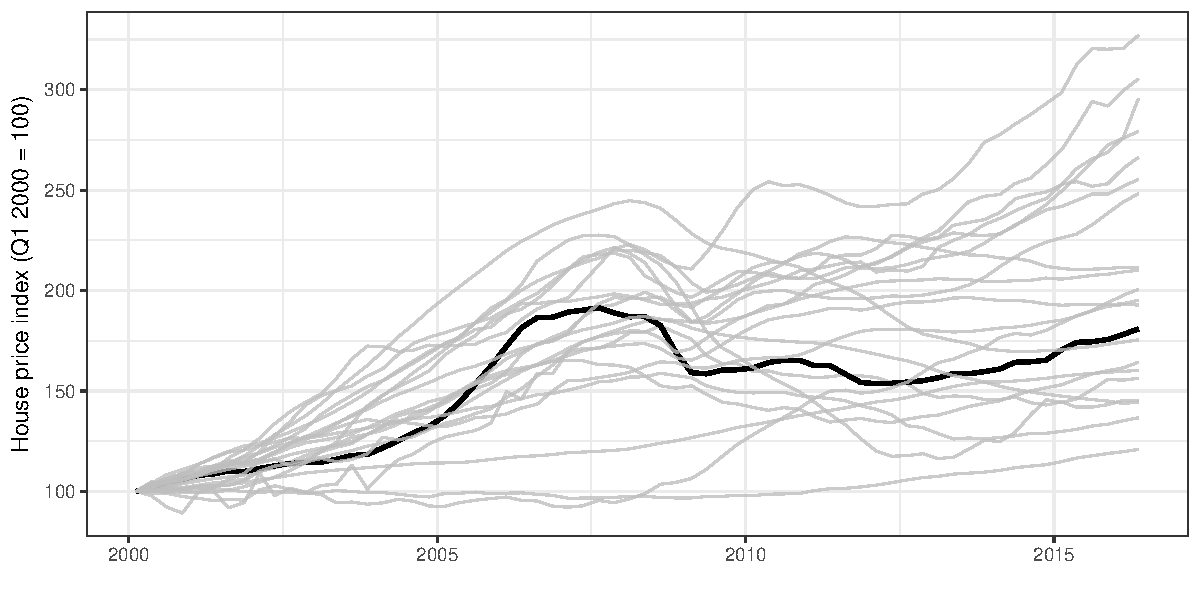
\includegraphics[width=0.9\textwidth]{../figures/timeplot}
		\centering
		\caption{Trends in real housing prices in Denmark (black line), Spain, the UK, and the US (dark gray lines) and selected other countries (light gray lines), 2000-2016 (2000 level = 100). Based on the International House Price Database maintained by the Dallas Fed. The authors acknowledge use of the dataset described in Mack and Martinez-Garcia (2011).}\label{hpd}
	\end{figure}
	Turning to the political context, the government in the period of our study (2002-2015) consisted of several different parties. From 2001 to 2011 the Liberal party formed a right-wing government along with the Conservative party, and from 2011 to 2015 the Social Democratic party formed a left-wing government together with the Social-Liberal Party and the Socialist People’s Party (the latter withdrew from the government in 2014). The fact that our study period covers governments led by parties from the centre-left and centre-right respectively is analytically advantageous as it enables us to differentiate local economic voting from other shifts in voter preferences. More specifically, because the policies exacerbating the housing bubble were introduced by the right-wing government holding office from 2001 to 2011, this renders support for the incumbent government observationally indistinguishable from voters becoming more ideologically conservative, a plausible consequence of increases in housing wealth \citep{ansell2014political}, in this period. By exploiting the change in incumbency in 2011-2015, we can ascertain that changes in local housing prices affect support for any incumbent government (local economic voting), and not merely support for a right-wing government (cf. Section \ref{inference}). 
	
	\section{Research design and data}\label{resdesign}
	Methodologically, we advance the study of local economic voting by exploiting comprehensive and highly granular data on housing market transactions available in Danish public registries. We link highly detailed registry data on local housing prices to both precinct-level panel data on national election outcomes as well as individual-level panel survey data (see below). These data ameliorate three methodological challenges confronting previous studies of the role of local economic conditions as well as the broader class of studies scrutinizing local influences on political attitudes and behavior.
	
	First, by utilizing precise and highly local measures of housing prices drawn from public registries we address the common problem of confounding local contexts with local media markets. Distinguishing between the two influences is rarely possible due to data constraints, specifically focusing on local economic conditions in more aggregated geographical contexts, where local context and local media markets overlap \citep[][]{bisgaard2016reconsidering}.  
	
	Second, and related to the previous point, measures of local economic conditions are often sample-based, which makes the estimation of conditions at lower geographical levels imprecise, thus causing attenuation bias (i.e. a downward bias) in the estimated relationship with support for the incumbent government \citep[][]{healy2017presidential}. We avoid such problems through the use of data from the full population, which enable us to measure local housing prices with very high precision.
	
	Third, most previous studies have relied on cross-sectional data \citep[e.g.,][]{reeves2012ecologies, ansolabehere2014mecro, books1999contextual}. While such data are often the best at hand, they come with the risk of confounding a relationship between local housing prices and support for incumbents by structural economic differences (e.g. differences in industry composition) between local contexts. This is perhaps best exemplified by the strong urban-rural gradient in local economic conditions, which would likely confound any observed cross-sectional relationship between such conditions and support for the sitting government. Using panel data, we can rule out confounding due to such time-invariant structural differences between local contexts by using only within-precinct/within-individual variation in local housing prices by means of precinct/individual fixed effects.
	
	Some previous studies address some of these methodological challenges, but our study is, to the best of our knowledge, the first to address all of these at once. In the remainder of this section, we present in more detail the two data sources we use two test our hypotheses; a precinct-level and an individual-level data set.
	
	\subsection{Precinct-level data and measures}\label{precinctlevel}
	We begin our analysis of the relationship between the state of local housing markets and incumbent support by looking at precinct-level election returns in Danish Parliamentary elections in 2005, 2007, 2011 and 2015. We match electoral support for parties in government in these precincts with change in the price of all house sales in and around the precincts, examining the extent to which local housing prices and local electoral support for government parties go hand in hand.
	
	The dependent variable in this analysis is \textit{percent of votes cast for government parties} in electoral precincts. Each voting precinct corresponds to a single polling place, which is the smallest unit at which voting returns can be observed in Danish elections. We measure this for all precincts in all four elections. There are roughly 1,400 precincts, each consisting of, on average, about 3,000 eligible voters and covering an area of 30 square kilometers. A number of precincts are redistricted between each election. This is problematic, as we want to use the precincts as part of a panel data set. One way to deal with this is to drop precincts as their geographical boundaries are altered. As a consequence, roughly 15 pct. of the data on the dependent variable would be dropped. We therefore opt for an alternative solution, namely to fix the precincts geographical boundaries at one reference election (2015), and then recalculate vote returns in any changed precincts to match up with precincts in the reference election. We prefer this strategy, allowing us to use the full sample of precincts, as the changes in geographical boundaries from election to election are generally minor with only a few major changes.\footnote{For details of how returns from the redistricted precincts are calculated, see Søren Risbjerg Thomsen's research note at \texttt{\href{http://bit.ly/205OlPi}{bit.ly/205OlPi}}.} The results presented below do not change substantially if we drop precincts that change boundaries, cf. Appendix \ref{calc}.
	
	We obtain data on the independent variable, local housing prices, from The Danish Mortgage Banks' Federation (\textit{Realkreditforeningen}), which publishes quarterly data on the average price per square meter of all sales at the zip code level, aggregated from registry data on individual sales.\footnote{Available at \texttt{\href{http://statistik.realkreditforeningen.dk/}{statistik.realkreditforeningen.dk}}.} We focus on changes in prices rather than price levels. This is motivated by the well-documented general tendency of human perceptions to be more responsive to changes in conditions than to absolute levels \citep{kahneman1979prospect}. It is also in keeping with the extant economic voting literature which, to the extent that it has looked at prices, has had a similar focus on changes (i.e., inflation, e.g. \citealp{kramer1971short}). At the local level, changes in housing prices will translate into shorter or longer turnaround times, as sellers and buyers try to adjust to the new prices, leaving visible traces of these changes in voters’ immediate context. These traces may take the form of ``for sale’’ signs in front yards and windows, or the speed at which old neighbors are exchanged for new ones. More precisely, we measure changes in housing prices as the percentage change in the price of houses sold in the quarter of a given election compared to the same quarter one year before. We merge observations of house prices and incumbent support by assigning every polling station to the year-on-year price change in its zip code. Additional details on this assignment procedure can be found in appendix \ref{app_linking}.
	
	To test \htwo, we measure local housing market activity by the (logged) number of trades in the zip code area (also based on data from The Danish Mortgage Banks' Federation). This is premised on the assumption that the number of trades in the zip code area manifests in various visible ways (e.g. more ‘for sale’ signs coming up and going down and a higher turnover in neighbors), which makes inhabitants more attuned to the state of their local housing markets and, in turn, makes support for the incumbent government (more) contingent on this part of the local economy.
	
	Finally, in the statistical models we control for the unemployment rate and median income at the zip-code level in order to isolate the effect of local housing markets from other features of the local economy. Like the independent variable, these are population-based measures calculated from public registries provided by Statistics Denmark.
	
	\subsection{Individual-level data and measures}\label{individuallevel}
	Although our precinct-level data is comprehensive, our hypotheses concern individuals, and testing individual-level theories with aggregate-level data is fraught with problems of ecological inference. Hence, we also analyze individual-level data from a two-wave panel survey collected between 2002 and 2011. The first wave of the panel survey consists of respondents who participated in round 1 (2002/3), 2 (2004/5) and 4 (2008/9) of the Danish Version of the European Social Survey (ESS); a nationally representative high-quality survey conducted bi-annually in most European countries.\footnote{\href{http://www.europeansocialsurvey.org/}{http://www.europeansocialsurvey.org/}} The second wave of the panel consists of re-interviewed respondents from these three rounds. Specifically, the full sample of ESS rounds 1 and 4, and 40 percent (randomly selected) of ESS round 2, were invited for a re-interview in the winter of 2011-12. In total, 1,745 people – equivalent to a retention rate of 47 pct. – were interviewed in both rounds.\footnote{The respondents for the ESS were (randomly) sampled from the Danish population registry, and therefore the civil registration numbers were retained by the data collection agency. This made it possible to identify the respondents for a second interview and to link the respondents to the national registers.} 
	
	From the survey, we use the following question as our dependent variable: ``What party did you vote for at the last parliamentary election?'' Respondents were presented with all the parties, which ran in the previous election. For the analyses we create a dummy variable indicating whether the respondent voted for a party in government at the time of the election as the dependent variable.\footnote{Since both survey waves are fielded shortly after national elections, reported party choice is temporally subsequent to economic changes over the past year.}
	
	We measure the independent variable, local housing markets, using data from the national Danish population registers, which are linked to the survey via anonymized civil registration numbers. The registers contain very detailed information about all individuals legally residing in Denmark, including the exact geographical location of their residence, the price of any real estate they sell, and a range of other socio-demographic characteristics \citep{thygesen2011introduction}. Important for our purposes, the registers make it possible to calculate the distance between the individuals in the survey and all other individuals in Denmark and, in turn, the distance to any individuals who are selling their home. Due to the detail and flexibility of the registry data, we can measure housing markets at a very local level, which, as discussed above,  allow for assessing the local economic conditions hypothesis at a much more theoretically appropriate level of analysis than in previous studies. If local economic voting can be observed based on very localized housing markets, it is a strong indication that local experiences are driving this relationship. 
	
	We measure local housing markets in three different ways and thereby address concerns related to the modifiable area unit problem (MAUP)—a thorny issue within contextual research in general—by examining whether our findings are tied to a particular geographic aggregation of housing prices. First, and similar to what we did for the precinct-level data, we use the respondents’ zip-code, comparing housing sold within the same zip code a year apart. Second, we look at the prices of the 20 or 40 units of housing sold closest to the respondents own home, comparing the prices of housing sold in the immediate proximity of the respondent to that of housing sold one year earlier. Third, we look at the price of housing sold within a fixed radius of 1000 or 1500 meters of the respondent. These latter ways of defining the respondents’ residential contexts have the benefit of being centered on the respondent, alleviating the problem that the context of a respondent living far from the centroid of one zip-code might be better represented by an adjoining zip-code. Note also that these latter two types of residential context differ in important ways: whereas the first method takes number of sales as fixed, but varies the geographical dispersion of these sales, the second method holds geographical dispersion fixed, but varies the number of sales. \footnote{See Appendix \ref{app_housingselect} for details of how we arrive at the housing price estimates.}
	
	More specifically, our independent variable is again year-over-year changes in housing prices in the residential context of the respondent. We measure the change by comparing the price of housing sold in the quarter prior to the data collection and the price of housing sold in the same quarter a year earlier. Unlike for the precinct-level data, we do not have data on prices per square meter. This makes the individual-level housing price change variable more sensitive to random variation in the types of housing put up for sale in the two time periods we compare. As such, year-to-year changes in prices may partly reflect that larger houses were put up for sale in a given year. To take this as well as other structural differences in the type of housing put up for sale into account, we divide the sales price of each unit of housing by its public valuation before calculating the year-over-year change. \footnote{The Danish government produces biannual estimates of the price of all housing in Denmark for the purpose of calculating property taxes. The public evaluation was constant across the time periods we use to estimate housing price changes.}
	
	Lastly, for evaluating \htwo, we develop a measure of individual-level involvement with the local housing market. We construct a variable from public registries whether the respondent moved within six months before or after being surveyed. The variable takes the value of one if respondents move within this period of time and zero otherwise. This variable can be viewed as a proxy for whether respondents are interacting with the housing market and thus whether they were exposed information about the trajectory of housing prices.
	
	We also include a number of additional variables in the analysis for statistical control, interaction analyses and placebo tests. We present these as we introduce them in the analysis. 
	
	\section{Precinct-level evidence} \label{inference}
	In the following, we present precinct-level evidence on our two hypotheses. Table \ref{predv}  evaluates the proposition that voters reward (punish) the incumbent government for increases (decreases) in local housing prices by means of a set of linear regression models. More specifically, the table presents the estimated effect of year-over-year changes in local housing prices on electoral support for the parties in government. All models are estimated using robust standard errors clustered at the precinct-level. Model 1 is a simple linear regression between electoral support and changes in housing prices. Model 2 includes year fixed effects, holding trends in incumbent support and rates of housing price changes constant. Model 3 adds precinct fixed effects to this specification, thus constituting a difference-in-difference model that evaluates whether increases in housing prices are related to incumbent support within precincts and net of any time trend (i.e., whether incumbent support increases more in precincts where housing prices increase more). In Model 4, we add the zip code-level unemployment rate and median income as covariates, thereby controlling for overall trends in the precincts’ economic situation. 
	
	\begin{table}[htbp]\centering
\def\sym#1{\ifmmode^{#1}\else\(^{#1}\)\fi}
\caption{Estimated effects of house prices on electoral support for governing parties.} \label{predv}
\begin{tabular}{l*{4}{c}}
\hline\hline
                    &\multicolumn{1}{c}{(1)}        &\multicolumn{1}{c}{(2)}        &\multicolumn{1}{c}{(3)}        &\multicolumn{1}{c}{(4)}        \\
\hline
$\Delta$ housing price&       0.104\sym{**}&       0.048\sym{**}&       0.053\sym{**}&       0.030\sym{**}\\
                    &     (0.008)        &     (0.007)        &     (0.008)        &     (0.007)        \\
[1em]
Unemployment rate   &                    &                    &                    &      -1.898\sym{**}\\
                    &                    &                    &                    &     (0.221)        \\
[1em]
Log(Median income)  &                    &                    &                    &      -0.891\sym{**}\\
                    &                    &                    &                    &     (0.064)        \\
[1em]
\hline Year FE      &                    &$\checkmark$        &$\checkmark$        &$\checkmark$        \\
[1em]
Precinct FE         &                    &                    &$\checkmark$        &$\checkmark$        \\
\hline
Observations        &        4193        &        4193        &        4193        &        4173        \\
RMSE                &       8.403        &       6.748        &       5.713        &       5.321        \\
\hline\hline
\multicolumn{5}{l}{\footnotesize Standard errors in parentheses}\\
\multicolumn{5}{l}{\footnotesize \sym{*} \(p<0.05\), \sym{**} \(p<0.01\)}\\
\end{tabular}
\end{table}

	
	Table \ref{predv} shows a statistically significant positive relationship between changes in housing prices and vote for the incumbent. In other words, consistent with the local economic conditions hypothesis, a larger fraction of the electorate casts their vote for governing parties in precincts where housing prices are increasing. 
	Notably, finding that the local unemployment rate is significantly negatively related to incumbent support in Model 4 is further support for the local economic conditions hypothesis. This also highlights that different aspects of the local economy matter independently of each other, rather than reflecting the same underlying economic conditions.
	
	Unsurprisingly, the effect of housing prices is larger in the less restrictive models. The effect size drops from 0.1 to 0.05 when introducing the time and precinct fixed effects, and drops additionally to 0.03 when introducing the economic controls. This highlights the strength of using a difference-in-difference approach and controlling for detailed information about other aspects of the local economy, as this evidently picks up important sources of confounding. In substantive terms, a coefficient of 0.03 implies that when the price of housing sold in a precinct's zip-code doubles from one year to the next, electoral support for governing parties in this precinct increases by roughly 3 percentage points. This corresponds to one third of a standard deviation in the dependent variable, and we might thus describe it as a modest but not negligible effect. The effect is also smaller, in absolute terms, than the effect of local unemployment. This is true even if we take into account that unemployment varies less than housing prices (cf. the descriptive statistics in Appendix \ref{sumstats}).  While it is hard to make straight-forward comparisons to existing work because results have been so inconsistent, this effect is also on the small side if we compare it to those estimated in \cite{healy2017presidential}. Here they find that moving from the 1st to the 99th percentile in local economic conditions (i.e., wage growth and loan delinquencies) increase incumbent support between 7 and 9 percentage points.

	Despite having employed a rigorous control strategy, a potential threat to our results is that that the effect of local housing markets on support for incumbents is a reflection of some secular trend predating changes in housing prices -- i.e., that governing parties were already becoming more/less popular in places where housing prices eventually increase/decrease. To address this concern about violation of the parallel trends assumption, we estimate the same type of models as in Table \ref{predv} using support for the governing party at the \textit{previous election} as the dependent variable (i.e. a lagged dependent variable). If we observe a significant relationship between prior support for incumbents and subsequent rises in housing prices, this would indicate that the parallel trends assumption is violated. We plot the estimated effects of housing prices on the lagged dependent variable as well as on the actual dependent variable in Figure \ref{placebo}. The figure shows a significant effect of housing prices on the lagged dependent variable in the less restrictive models. However, in the final and most restrictive model, the estimated effect of housing prices on lagged incumbent support is 0.005 -- less than a sixth of the estimate on subsequent support -- and statistically insignificant. This indicates that trends in incumbent support are similar across precincts where prices are about to increase and precincts where prices  are about to decrease. That is, pre-‘treatment’ trends in treated and non-treated units are likely parallel.
	
	\begin{figure}[htbp!]
		\includegraphics[width=0.9\textwidth]{../figures/lagdv.eps}
		\centering
		\caption{Effects of Housing Prices on support for governing party at the present election (t) and the last election (t-1) with 90  and 95 pct. confidence intervals}\label{placebo}
	\end{figure}
	
	We proceed to evaluate \htwo, testing whether the relationship between changes in local housing prices and incumbent support is moderated by local housing market activity. Table \ref{table:econactivity} reports a set of models similar to those presented in Table \ref{predv}, but with changes in housing prices interacted with the (logged) number of trades in the preceding quarter as an indicator of housing market activity. As noted previously, we expect greater local housing market activity to manifest itself locally in various visible ways (e.g. neighbors selling their houses more rapidly), which in turn makes housing prices more salient and thus consequential for voters’ support for incumbents. Consistent with the contextual priming hypothesis, we observe a statistically significant positive interaction between local housing prices and housing market activity in all models. That is, local housing prices are more strongly related to incumbent support in areas with higher levels of housing market activity..
	
	\begin{table}[htbp]\centering
\def\sym#1{\ifmmode^{#1}\else\(^{#1}\)\fi}
\caption{Estimated effects of housing price across number of trades.} \ref{table:econactivity}} \label{prelagiv}
\begin{tabular}{l*{4}{c}}
\hline\hline
                    &\multicolumn{1}{c}{(1)}        &\multicolumn{1}{c}{(2)}        &\multicolumn{1}{c}{(3)}        &\multicolumn{1}{c}{(4)}        \\
\hline
$\Delta$ housing price&      -0.039        &      -0.102\sym{**}&      -0.077\sym{**}&      -0.079\sym{**}\\
                    &     (0.027)        &     (0.021)        &     (0.023)        &     (0.023)        \\
[1em]
$\Delta$ housing price $\times$ logntrades&       0.049\sym{**}&       0.050\sym{**}&       0.038\sym{**}&       0.033\sym{**}\\
                    &     (0.008)        &     (0.007)        &     (0.007)        &     (0.007)        \\
[1em]
Unemployment rate   &                    &                    &                    &      -1.656\sym{**}\\
                    &                    &                    &                    &     (0.217)        \\
[1em]
Log(Median income)  &                    &                    &                    &      -0.856\sym{**}\\
                    &                    &                    &                    &     (0.063)        \\
[1em]
\hline Precinct FE  &                    &                    &$\checkmark$        &$\checkmark$        \\
[1em]
Year FE             &                    &$\checkmark$        &$\checkmark$        &$\checkmark$        \\
\hline
Observations        &        4195        &        4195        &        4195        &        4175        \\
RMSE                &       8.501        &       6.736        &       5.637        &       5.288        \\
\hline\hline
\multicolumn{5}{l}{\footnotesize Standard errors in parentheses}\\
\multicolumn{5}{l}{\footnotesize \sym{*} \(p<0.05\), \sym{**} \(p<0.01\)}\\
\end{tabular}
\end{table}

	
	Since interaction models can be difficult to interpret based on reported coefficients alone, we visualize the result in Figure \ref{localactivity}. For each model specification, the figure shows the predicted effect of local housing prices on incumbent support for zip code economic activity corresponding to the 25\textsuperscript{th} and 75\textsuperscript{th} percentile. Focusing on the most restrictive model, the most notable result is that for the most restrictive model, there is essentially no effect of local housing prices at the bottom 25\textsuperscript{th} percentile of local housing market activity, while the effect is about twice the size of the average effect  (i.e., 0.06) at the 75\textsuperscript{th} percentile. The latter corresponds to electoral support for governing parties increasing by roughly 6 percentage points in a precinct, where house prices in the zip-code area doubles from one year to the next. Interestingly, the effect at the 75th percentile is more in line with the findings in \citep{healy2017presidential}described above. We thus find clear support for \htwo. In localities where the local housing market is more active, and thus ostensibly more salient to voters, housing prices feature more prominently in the evaluation of incumbents. 
	
	One potential concern in relation to this analysis is that housing prices and market activity measure the same underlying phenomenon, complicating the interpretation of the interaction term. However, as we show in Appendix \ref{app_interaction}, the two are in fact very weakly correlated ($r=0.1$), implying that they essentially vary independently of one another. Another concern is that number of trades is a proxy for population size. To test this, we estimate a model which includes an interaction between housing prices and logged number of eligible voters in the precinct as well as the interaction with number of trades. In this model, we find no significant interaction with population size, and the remains statistically significant and of the same approximate size, suggesting that our results are driven by variation in market activity which is independent of market size. These results are reported in Appendix \ref{add_interaction}.
	
	We made no prediction about whether contextual priming of local housing markets would lessen the effect of other economic conditions, however, if one accepts that voter attention is limited, one might think that it would do just that \citep[this is a common assertion in the broader priming literature, see for instance][]{krosnick1990altering}. In Appendix \ref{add_interaction} we tentatively examine whether this is the case by interacting our measure of local housing market activity with the unemployment rate. We find that unemployment does seem to matter a bit less when the local housing market is more active, however, the pattern is less pronounced than for the housing price interaction.  
	
	
	\begin{figure}[htbp!]
		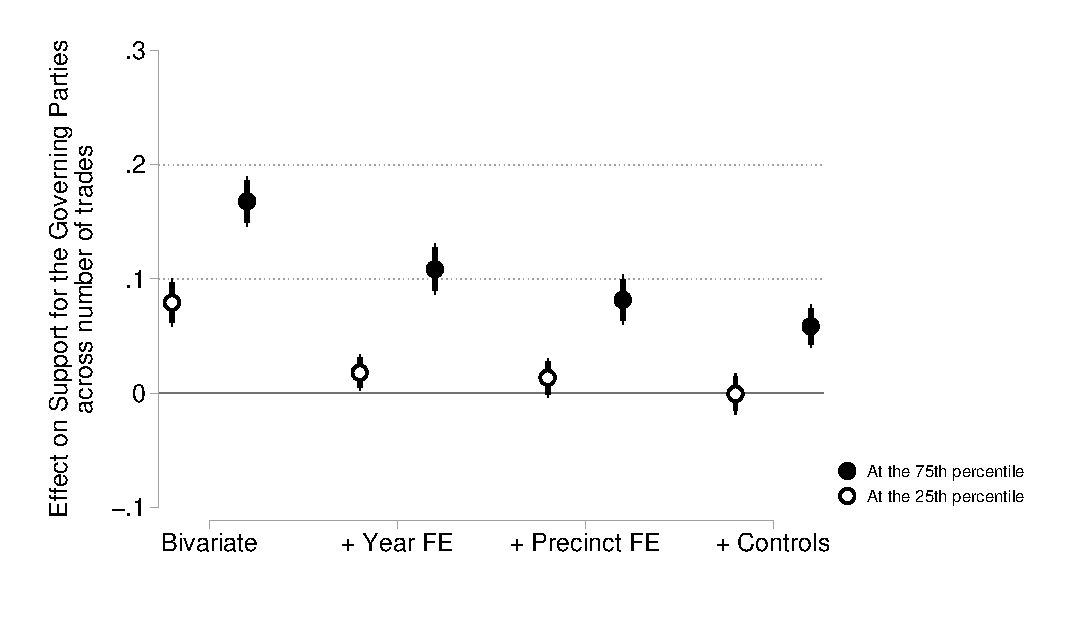
\includegraphics[width=0.9\textwidth]{../figures/localactivity.eps}
		\centering
		\caption{Marginal effects of housing prices across levels of economic activity with 90 and 95 pct. confidence intervals.  Marginal effects derived based on table \ref{table:econactivity} at the 25th and 75th percentile.}\label{localactivity}
	\end{figure}
	
	
	
	\subsection{Auxiliary analyses and robustness checks}
	Table \ref{robustness} presents a series of robustness checks of the results presented above. For these analyses, we only report the estimated average effect of housing prices and the interaction between (logged) number of trades and housing prices. The full models are reported in Appendix \ref{app_robustpred} of the supplementary materials.
	
	\begin{table}[htbp]\centering
	\def\sym#1{\ifmmode^{#1}\else\(^{#1}\)\fi}
	\caption{Assesing the Robustness of the Precinct-level Evidence} \label{robustness}
	\begin{tabular}{l*{4}{c}}
		\hline\hline
		&\multicolumn{1}{c}{(1)}        &\multicolumn{1}{c}{(2)}        &\multicolumn{1}{c}{(3)}        &\multicolumn{1}{c}{(4)}        \\
\hline
$\Delta$ housing price (2 years)&       0.129\sym{**}&       0.037\sym{**}&       0.022\sym{**}&       0.020\sym{**}\\
&     (0.007)        &     (0.007)        &     (0.007)        &     (0.007)        \\
[1em]
$\Delta$ housing price (FD controls)&       0.104\sym{**}&       0.073\sym{**}&       0.086\sym{**}&       0.058\sym{**}\\
&     (0.008)        &     (0.008)        &     (0.009)        &     (0.008)        \\
[1em]
$\Delta$ housing price (FD DV)&       0.037\sym{**}&       0.034\sym{**}&       0.052\sym{**}&       0.019\sym{**}\\
&     (0.004)        &     (0.004)        &     (0.005)        &     (0.004)        \\
[1em]
$\Delta$ housing price (negative)&      -0.081\sym{***}&      -0.072\sym{***}&      -0.057\sym{**} &      -0.030         \\
&     (0.022)         &     (0.017)         &     (0.019)         &     (0.019)         \\
[1em]
$\Delta$ housing price (positive)&       0.116\sym{***}&       0.045\sym{***}&       0.031\sym{**} &       0.029\sym{*}  \\
&     (0.012)         &     (0.011)         &     (0.011)         &     (0.011)         \\
[1em]
\hline Economic controls  &                    & $\checkmark$                    &$\checkmark$        &$\checkmark$        \\
[1em]
Precinct FE  &                    &                    &$\checkmark$        &$\checkmark$        \\
[1em]
Year FE             &                    &                    &                    &$\checkmark$        \\
\hline\hline
\multicolumn{5}{l}{\footnotesize Standard errors in parentheses}\\
\multicolumn{5}{l}{\footnotesize \sym{*} \(p<0.05\), \sym{**} \(p<0.01\)}\\
\end{tabular}
\end{table}
	
	We begin by looking at whether the chosen time period, i.e. year-over-year changes, affects the results. To do so, we re-estimate the most restrictive model from tables \ref{predv}--\ref{table:econactivity} using the change in housing prices over two years rather than just one. The results, reported in the first row in Table \ref{robustness}, are similar using this measure of more long run changes in housing prices, although the estimated effects tend to be smaller than reported above. This squares with previous work showing that voters are, by and large, myopic when it comes to relating economic indicators to incumbent support \citep{healy2009myopic,healy2014substituting}.
	
	As mentioned above, we use changes in housing prices rather than levels. However, in our models we control for the level of income and the level of unemployment. As a consequence, we may fail to capture something important about how the economic status of the precinct is changing, which could in turn confound the effect of changes in housing prices. To examine whether this is the case, we re-estimate the different models using first-differenced (FD) controls. As can be seen in the second row of Table \ref{robustness}, this does not alter the main conclusion. In fact, the estimated effects of local housing prices doubles in size in this specification. We also estimate a set of complete change models using an FD dependent variable. The estimates from these models are reported in the third row of Table \ref{robustness}. While somewhat smaller, the effect of housing prices remains statistically significant in the differenced model.
	
	To test for nonlinearities in the observed relationship, we split the housing price variable in two, creating one variable measuring the size of positive changes with negative changes set to zero, and another one measuring the size of negative changes with positive changes set to zero. This makes it possible to study the effect of increases and decreases in housing prices separately. We report the result of these analyses in the last two rows of Table \ref{robustness}. Interestingly, we find no evidence of negativity bias: the effect of negative changes and positive changes are both roughly 0.03 in absolute numbers. This symmetry is important because it shows that voters not only reward governing politicians when housing prices are on the rise, but also punish them when they fall. Moreover, the effect of both positive and negative changes are both conditioned by the number of trades.  This contrasts with earlier studies finding that voters respond more strongly to negative economic changes \citep[e.g.][]{bloom1975voter,headrick1991attention,soroka2014negativity}. 
	
	Another concern relates to whether the effect is only present for right-wing incumbents. As housing prices in an area increases, the wealth of the voters living in this area also increases on average, which might lead to increased support for right-wing politicians \cite{ansell2014political}. This problem is especially acute in our data, as the government parties in power from 2001 to 2011 were right-wing. To address this concern, we estimate models predicting support for the left-wing government coalition (Social Democrats and the Social-Liberal Party) and the right-wing government coalition (Liberal Party and Conservative Party) using housing prices, precinct and year fixed effects, as well as the local economic controls. We then interact the housing prices measure with a binary indicator for whether the parties are in office.\footnote{We estimated this model on a dataset which included all precinct-years twice: once with the left-wing coalition support and once with right-wing coalition support. The housing price effect is conditioned on a two-way interaction between government coalition (i.e., whether we are predicting support for left-wing or right-wing government coalition) and whether this coalition is in office. See Appendix \ref{app_partyspec} in the supplementary materials for the full model.} Figure \ref{partyspecific} presents the key estimates from this model. As shown, increasing housing prices have a positive estimated effect on electoral support for right-wing as well as left-wing incumbent government parties. Our result can thus not be explained by increased housing wealth causing a conservative shift in the electorate. In other words, the relationship between changes in local housing prices and support for incumbent governments is independent of the partisan composition of the government.
	
	\begin{figure}
		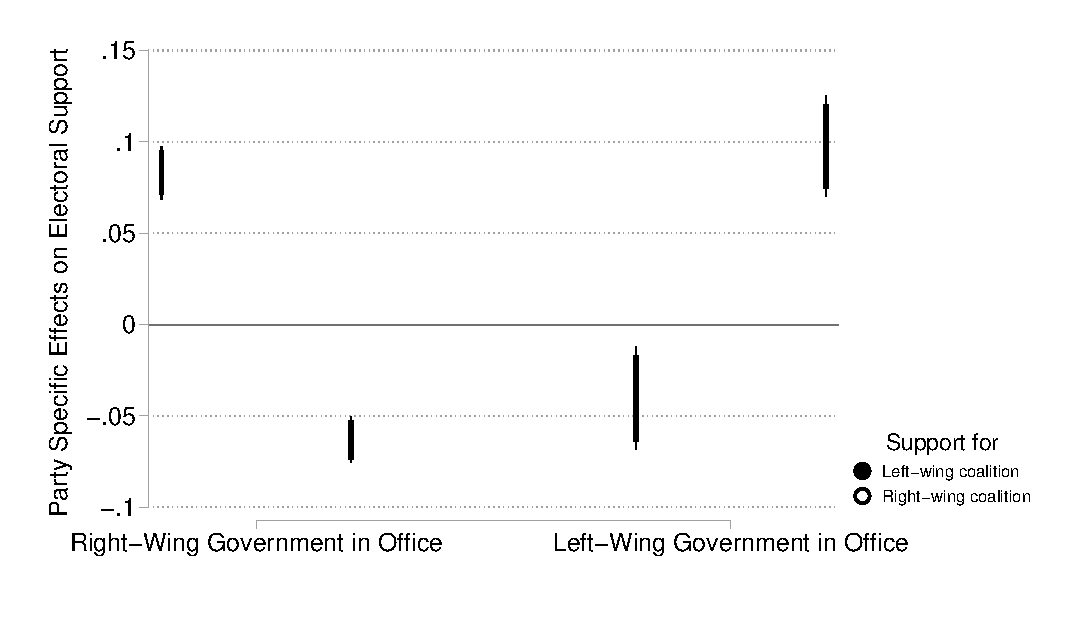
\includegraphics[width=1\textwidth]{../figures/partyspecific.eps}
		\caption{The marginal effect of housing prices on electoral support for either the left-wing or the right-wing government coalition conditional on which coalition is in office. See Appendix \ref{app_partyspec} of the supplementary materials for the model underlying this figure. Error bars represent 90 and 95 pct. confidence intervals.}
		\label {partyspecific}
	\end{figure}
	
	Finally, one might suspect that the interaction term is non-linear. Using the binning estimator presented in \cite{hainmueller2016much}, we find some evidence of this, as the effect of housing prices only seems to materialize in the upper tercile of the moderator. We present this analysis in Appendix \ref{app_interaction}. However, even when relaxing the linearity constraint on the moderator, the observed relationship is consistent with \htwo in that we did not specify that the relationship between local housing market activity and the effect of housing prices was monotonically increasing. 
	In sum, we find clear evidence for both \hone and \htwo in the precinct-level data. We now proceed to testing the hypotheses using the individual-level data, and thus get a stronger hold of the purported individual-level mechanisms at play.
	
	\section{Individual-level evidence}
	
	In Table \ref{inddv} we report results from a set of linear probability models, estimating the probability of voting for a party in government as a function of changes in local housing prices. We choose to estimate linear probability models in the interest of simplicity, but we show in Appendix \ref{app_robustind} that the results are virtually identical when estimated using conditional logistic regression models. We include individual (respondent) fixed effects, and fixed effect for which of the four different survey rounds the respondent initially participated in (ESS rounds 1, 2 or 4). All models include controls for the average income and unemployment rate in the respondent's context, as well as indicators of the respondent's own income and whether someone in the household is unemployed. Like in the precinct-level analyses, we include these controls to isolate the effect of local housing markets from trends in overall economic circumstances. However, unlike for the precinct-level data, we can now control for trends in both the respondent’s personal economy and for the economy of her larger social context. In effect, we utilize a similar identification strategy as for the precinct-level data: a difference-in-difference model that controls for trends in economic conditions. All models include robust standard errors clustered at the individual-level.
	
	All models include the same set of variables, but differ in how the contextual variables are defined. In column one we present a model where housing price change is calculated based on the 20 sales closest to each respondent, and where the other contextual variables -- average income and unemployment rate -- are measured within a 500 meter radius of each respondent. In column two we use the 40 closest sales, but leave the remaining variables measured as in column one. In columns three and four we define all contextual variables (house prices, unemployment rate and average income) as based on 1000 and 1500 meter radii around the respondent. Finally, in column five, we examine sales at the level of zip code areas. 
	
	\begin{table}[htbp]\centering
\def\sym#1{\ifmmode^{#1}\else\(^{#1}\)\fi}
\caption{Linear Regression of Voting for Governing party } \label{inddv}
\begin{tabular}{l*{5}{c}}
\hline\hline
                    &\multicolumn{1}{c}{20 Closest}&\multicolumn{1}{c}{40 Closest}&\multicolumn{1}{c}{1000 metres}&\multicolumn{1}{c}{1500 metres}&\multicolumn{1}{c}{Zip code}\\
\hline
$\Delta$ housing prices&       0.035       &       0.056       &       0.064       &       0.114\sym{*}&       0.063       \\
                    &     (0.036)       &     (0.044)       &     (0.052)       &     (0.051)       &     (0.056)       \\
[1em]
Unemployment rate   &       0.052       &       0.056       &      -0.439       &       0.755       &       0.796\sym{+}\\
                    &     (0.290)       &     (0.289)       &     (0.627)       &     (0.575)       &     (0.422)       \\
[1em]
Average income      &      -0.004       &      -0.004       &      -0.005       &      -0.005       &      -0.006       \\
                    &     (0.003)       &     (0.003)       &     (0.007)       &     (0.007)       &     (0.006)       \\
[1em]
Personal income     &      -0.000       &      -0.000       &      -0.000       &      -0.000       &      -0.000       \\
                    &     (0.000)       &     (0.000)       &     (0.001)       &     (0.001)       &     (0.000)       \\
[1em]
Unnemployed (household)&      -0.032       &      -0.033       &      -0.066       &      -0.048       &      -0.034       \\
                    &     (0.035)       &     (0.035)       &     (0.043)       &     (0.040)       &     (0.036)       \\
[1em]
\hline  Round FE    &         Yes       &         Yes       &         Yes       &         Yes       &         Yes       \\
[1em]
Individual FE            &         Yes       &         Yes       &         Yes       &         Yes       &         Yes       \\
\hline
Observations        &        3479       &        3479       &        2790       &        2992       &        3384       \\
\hline\hline
\multicolumn{6}{l}{\footnotesize Standard errors in parentheses}\\
\multicolumn{6}{l}{\footnotesize \sym{+} \(p<0.1\), \sym{*} \(p<0.05\)}\\
\end{tabular}
\end{table}

	
	The estimated effect of changes in local housing prices is positive across the different models, although the size of the coefficient varies somewhat, ranging from 0.04 to 0.11. The effect is only statistically significantly different from zero in the specification measuring sales within 1500 meters of the respondent.
	
	While we only observe a statistically significant relationship between changes in housing prices and voting for the incumbent in one out of five models, it is important to highlight that the estimated relationships are consistent with what we found in the precinct-level data. To illustrate this, Figure \ref{comparison} plots the estimated effect of housing prices estimated for the individual-level data in Table \ref{inddv} and for the precinct-level data in Table \ref{predv}.
	
	\begin{figure}[htbp!]
		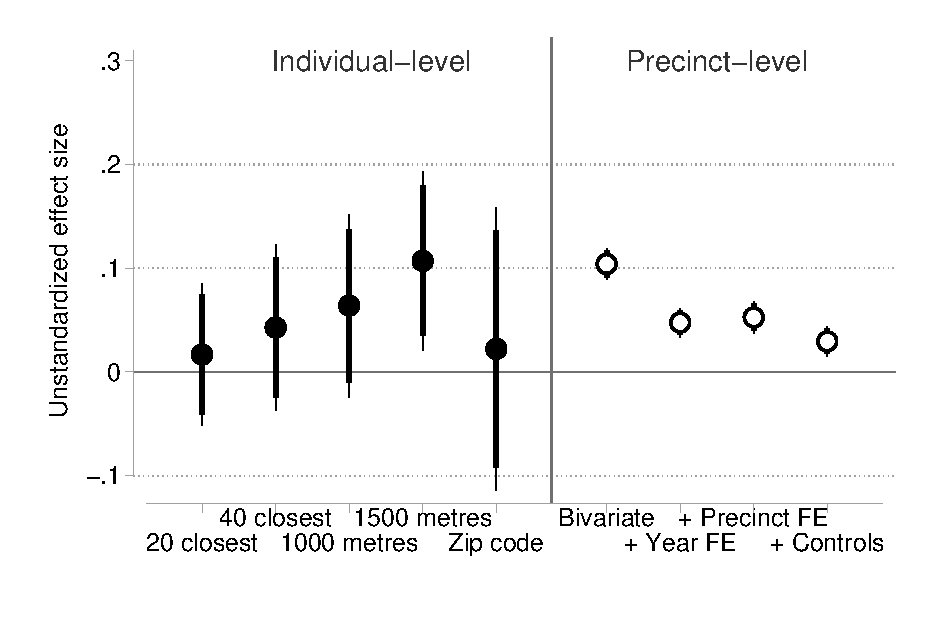
\includegraphics[width=0.9\textwidth]{../figures/comparison.eps}
		\centering
		\caption{Effects of Housing Prices across levels of analysis with 90 and 95 pct. confidence intervals}\label{comparison}
	\end{figure}
	
	As is clear from the figure, the effect sizes are similar across the two levels of analysis. If anything, the estimated effects appear slightly larger for the individual-level data. This tentatively suggests that that the estimated coefficients do not represent a true null effect, but rather an imprecisely estimated one. One plausible reason for this imprecision is measurement error in the dependent variable as voter recall data are known to be erroneously reported \citep[e.g.,][]{bernstein2001overreporting}. In sum, we find mixed support for \hone in the individual-level data, as the effect of housing prices is statistically insignificant in most specifications, but comparable in sign and magnitude to the precinct-level results.
	
	We now test \htwo using the individual level data. Following our contextual priming-argument, we expect those who recently interacted with their local housing market to have considerations regarding local housing more readily available when evaluating the incumbent government. One such group is those who have just moved or who are on the cusp of moving, as they are currently, or have recently, been exposed to information regarding local housing markets as a result of selling their present home and looking for a new one. 
	
	Table \ref{tabmovers} presents a set of re-estimated individual-level models from table \ref{inddv}, where the the housing price change variable is interacted with an indicator for whether or not the respondent is a mover (i.e., those who moved six months before/after being surveyed). The estimated interaction effect is statistically significant and positive in all specifications ($p<.05$ for all models except the zip-code model, $p<.1$ for the zip-code model), thus  showing that the group of movers are in fact significantly more responsive to changes in local housing prices. 
	
	Figure \ref{move} presents marginal effects for movers and non-movers derived from the models in Table \ref{tabmovers}. As shown, housing prices have large significant ($p<.05$) estimated effects for movers and a negligible effect—often essentially no effect—for non-movers. For movers, the effect of changes in housing prices is estimated to be between 0.2 and 0.4 depending on the model. In substantive terms, this means that when housing prices double the probability of voting for the incumbent increases by 20 to 40 percentage points for voters who are currently involved with local housing market. This is quite a large effect, much larger than even the largest effects identified in the previous literature on local economic voting \citep{healy2017presidential}, which suggests that when an individual is attuned to a part of their local economy, this part of the economy plays an essential role in their decision to support the national government. Because of the large sampling variability, we cannot say anything about whether the effect is larger at any particular level of aggregation, however, it is reassuring that we find the same overall pattern across these different levels of aggregation (cf. the MAUP). 
	Overall, these results strongly support the contextual priming hypothesis by showing that changes in local housing prices play a larger role in incumbent evaluations among individuals who been more exposed to their local housing market though their interaction with it.
	
	\begin{table}[htbp]\centering
\def\sym#1{\ifmmode^{#1}\else\(^{#1}\)\fi}
\caption{Linear Regression of Voting for Governing party } \footnotesize \label{tabmovers}
\begin{tabular}{l*{5}{c}}
\hline\hline
                    &\multicolumn{1}{c}{20 Closest}&\multicolumn{1}{c}{40 Closest}&\multicolumn{1}{c}{1000 metres}&\multicolumn{1}{c}{1500 metres}&\multicolumn{1}{c}{Zip code}\\
\hline
$\Delta$ housing prices&      -0.005       &       0.021       &       0.040       &       0.086\sym{+}&      -0.010       \\
                    &     (0.038)       &     (0.044)       &     (0.046)       &     (0.046)       &     (0.073)       \\
[1em]
Mover               &       0.010       &       0.012       &       0.004       &       0.025       &       0.030       \\
                    &     (0.030)       &     (0.031)       &     (0.036)       &     (0.032)       &     (0.031)       \\
[1em]
$\Delta$ housing prices $\times$ Mover&       0.180\sym{*}&       0.233\sym{*}&       0.266\sym{*}&       0.304\sym{*}&       0.377\sym{*}\\
                    &     (0.084)       &     (0.108)       &     (0.121)       &     (0.111)       &     (0.148)       \\
[1em]
Unemployment rate (context)&       0.260       &       0.259       &      -0.491       &       0.740       &       0.772\sym{+}\\
                    &     (0.374)       &     (0.375)       &     (0.634)       &     (0.586)       &     (0.421)       \\
[1em]
Average income (context)&      -0.002       &      -0.002       &      -0.005       &      -0.004       &      -0.005       \\
                    &     (0.004)       &     (0.004)       &     (0.007)       &     (0.007)       &     (0.006)       \\
[1em]
Personal income     &      -0.000       &      -0.000       &      -0.000       &      -0.000       &      -0.000       \\
                    &     (0.000)       &     (0.000)       &     (0.001)       &     (0.001)       &     (0.000)       \\
[1em]
Unnemployed (household)&      -0.034       &      -0.034       &      -0.070       &      -0.054       &      -0.033       \\
                    &     (0.035)       &     (0.035)       &     (0.043)       &     (0.040)       &     (0.036)       \\
[1em]
\hline  Round FE    &         Yes       &         Yes       &         Yes       &         Yes       &         Yes       \\
[1em]
Voter FE            &         Yes       &         Yes       &         Yes       &         Yes       &         Yes       \\
\hline
Observations        &        3479       &        3479       &        2790       &        2992       &        3392       \\
\hline\hline
\multicolumn{6}{l}{\footnotesize Standard errors in parentheses}\\
\multicolumn{6}{l}{\footnotesize \sym{+} \(p<0.1\), \sym{*} \(p<0.05\)}\\
\end{tabular}
\end{table}

	
	\begin{figure}[htbp!]
		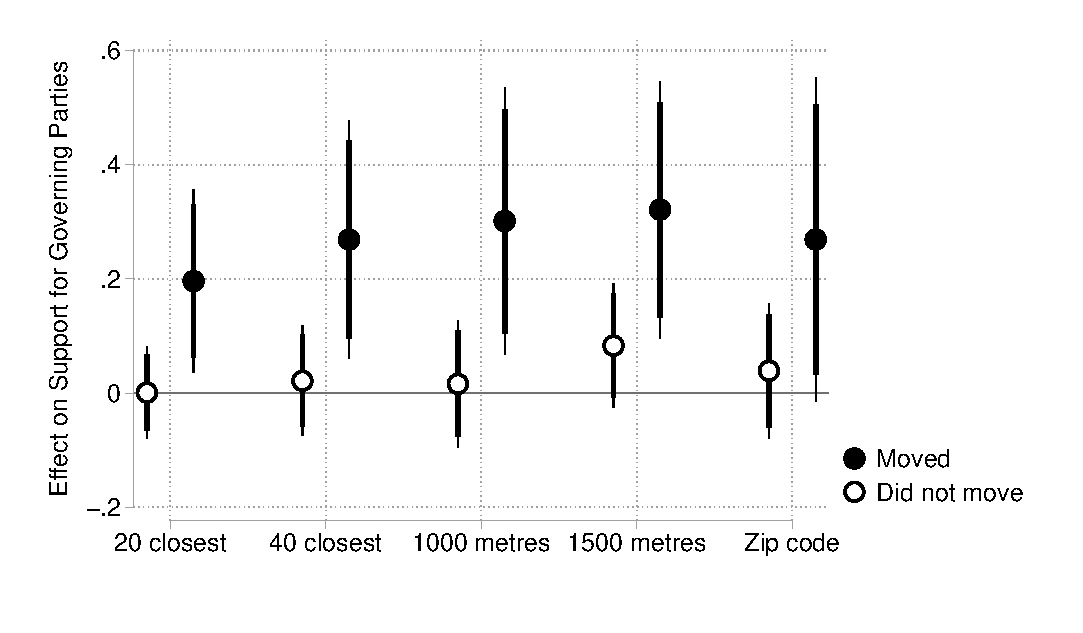
\includegraphics[width=0.9\textwidth]{../figures/moving.eps}
		\centering
		\caption{Effects of Changes in Housing Prices for those who had just or were going to move and those who did not with 90 and 95 pct. confidence intervals}\label{move}
	\end{figure}
	
	
	\subsection{Auxiliary analyses and robustness checks}
	
	Although the individual-level data are more constrained in terms of number of observations and number of time periods, we also conducted a number of supplementary analyses of these (see Appendix \ref{app_robustind} for detailed results of these additional analyses). For one, we tried to re-estimate the models using a conditional logit model (i.e. logit with unit fixed effects). This takes into account that the dependent variable is dichotomous, but also entails that all observations that do not change voting behavior between the two periods are omitted from the sample. These logit models reveal the same basic pattern as the linear models. 
	
	We also examined whether the effect of local housing prices vay by home ownership status. In most models we find positive, yet statistically insignificant interactions. While this may be seen as a weak indication that local housing markets are somewhat more salient to those more financially involved with them, we think that the more proper conclusion to draw is that cues about the state of the local economy diffuse from the local context independently of strong personal involvement. 
	Finally, following the party-specific analysis for the precinct-level data, which explored whether voters’ responses to local economic conditions had an ideological bent, we look at whether changes in local housing prices affect voters self-placement on a ten point left to right ideological scale. The estimated effects are generally small, statistically insignificant, and negative, suggesting that if anything, voters become more left-wing as housing prices increase. This again runs counter to the notion that our findings can be explained by voters responding to increases in local housing prices by become more  conservative.
	
	Taken together, consistent with our hypotheses, the individual-level analyses suggest that voter’s decision to support the sitting government is partly based on changes in local housing prices (\hone), and even more so for those individuals particularly attuned to the housing market (\htwo). 
	
	\section{Discussion and conclusion}
	Following  the lead of previous efforts, this paper  has examined the phenomenon of local economic voting—the notion that voters in part base their electoral support for national governments on the economic situation in their local community. We have proposed and empirically tested two hypotheses. First, the local economic conditions hypothesis stating—in line with previous studies—that local economic conditions affect support for incumbent governments. Second, the contextual priming hypothesis, which suggests that local economic conditions are more salient to voters, who are more exposed to it, and therefore more consequential for their support for incumbents. 
	
	Using exceptionally precise and flexible registry data on local housing markets from Denmark during the housing bubble preceding  the Great Recession, we find support for both hypotheses.More specifically, we merge precinct-level panel data on election outcomes and individual-level panel survey data on vote choice with the registry data on local housing markets.
	
	We find strong support for the economic conditions hypothesis in the precinct-level data and also, more tentatively, in the individual-level data. In the precinct-level data, a 50 percent year-on-year increase in local housing prices translates into a 1 to 2 percentage point increase in electoral support for the governing parties. Findings from both the precinct-level data and the individual-level data support the contextual priming hypothesis. In precincts with higher economic activity, local house prices are more consequential for voters’ support for the incumbent. Similarly, among individuals who are exposed to the housing market through the process of selling a home, local house prices figure more prominently in their evaluation of the incumbent government. In short, local economic voting based on the fate of local housing markets does occur, and more prominently so when this aspect of the local economy is more salient to voters.
	
	While we believe that our data are very well suited for testing the proposed hypotheses and constitute a clear improvement over previous related studies in several regards, a number of caveats are warranted. First, our data are observational and in the absence of fully or quasi-experimental variation in housing prices, we cannot be sure that the estimated effects are not confounded by unobserved heterogeneity. Building on this study, one promising avenue for future research is therefore to identify settings with plausibly exogenous variation \citep{jerzak2016property}. Second, while our overall result regarding the existence of local economic voting confirms findings from other countries (in more aggregate local contexts), we cannot know whether our novel finding regarding contextual priming travels to other contexts. A priori, we have no reasons to expect this finding to be idiosyncratic to Denmark, but this remains an empirical question. 
	Our results carry several implications for the literature on economic voting in particular as well as research on political behavior in general. Most obviously, with regard to the former, our study adds to the mounting evidence of local economic voting. Consistent with existing studies, we find modest, but non-negligible effects \cite{healy2013retrospective} of local economic context on support for the incumbent government. However, we do so using data from highly localized contexts rather than more aggregate contextual units, where local experiences may be confounded by other factors. This speaks to the fruitfulness of further exploration of how cues of economic performance experienced very locally, influence incumbent support and other evaluations and beliefs related to national politics \citep[e.g.,][]{burnett2017politics}.
	
	In this paper, we have focused on local housing markets, but our theoretical arguments concern the importance of local economic context more generally. As noted, we also find a significant (negative) effect of local unemployment on support for incumbents in the precinct-level data, which shows that local economic conditions are a multifaceted phenomenon. This suggests that examining which aspects of the local economy shape electoral support for the sitting government at a given point in time—and the potential interplay between them—is a fruitful next step in the analysis of local economic voting. This may also provide further leverage for refining our contextual priming hypothesis. One implication of classical theories of priming is that once one set of concerns become salient other concerns fade \citep{ krosnick1990altering}. Similarly, we may expect that when one aspect of the local economic context takes center stage due to voters’ involvement with it, other aspect of the local economy diminish in importance. The precinct-level data reveal a pattern consistent with this conjecture. Whereas local housing prices become much more important for support for the incumbent government in contexts with highly active housing markets, the effect of local unemployment drops somewhat (although not significantly) in these contexts. We believe this is an interesting conjecture that could be tested further in future work to advance our understanding of when certain aspects of the local economy matter for local economic voting.
	
	In relation to the priming literature within political psychology, our results indicate that priming does not only happen as the result of elite messaging, but may also stem from personal involvement with a specific aspect of society, in our case local housing markets. Exploring other `sideways’ sources of priming of predispositions including various personal experiences would provide a nice complement to the heavy focus on elite-driven (‘top down’) media influences presently characterizing the priming literature. 
	
	What does voters’ use of local housing markets as a shorthand for evaluating national incumbents tell us about the nature of voters’ motives and democratic accountability? As noted, in the individual-level data we find that local economic voting occurs largely independently of home ownership status. This in turn suggests that local economic voting primarily reflects sociotropic—whether related to the local community or the nation as a whole—rather than personal financial (egotropic) concerns. However, our findings are ambiguous as to whether local economic voting is an effective heuristic for holding national politicians accountable. On the one hand, using local economic conditions to inform voting can be seen as an economic way for voters to reward or punish the national government for progress or hardship they experience in their local environment. Yet, on the other hand, such local developments may be a weak signal of overall government performance.
	
	Finally, on a more substantive note, our findings suggest that local economic voting is adaptive rather than static. Voters do not seem transfixed by certain parts of their local economy, such as unemployment or housing prices. Instead, they focus on the parts of the economy, which they are currently involved with. It is unclear whether this is good or bad news in the context of electoral accountability. On one hand, this undoubtedly means that voters will often get a very selective and unreliable impression of  local economic conditions. As such, two voters who live in the same local context might arrive at wildly different impression of their local economy depending on whether they are engaged in a job search or a search for a new house.  On the other hand,  it is clearly positive that voters are able to refocus their attention towards new parts of the economy, such as the housing market, as they become relevant to their own lives. If they did not, reelection-oriented incumbents would not have any incentive to take care of these new parts of the economy.
	

	
	\clearpage
	
	\singlespacing
	
	\bibliographystyle{apa}
	\bibliography{library}
	
	\newpage
	
	\appendix
	\section*{Appendix}
		\onehalfspacing
	\renewcommand{\thesubsection}{\Alph{subsection}}
	\renewcommand{\thetable}{\Alph{subsection}\arabic{table}}
	\renewcommand{\thefigure}{\Alph{subsection}\arabic{figure}}
	
	\localtableofcontents

	
	\newpage
	
	\subsection{Linking Polling Places to Zip Codes}\label{app_linking}
	
	Zip codes are a substantively interesting level of aggregation when it comes to the price of housing, as it is the level at which housing prices are most often reported in Denmark (cf. the fact they are published by The Danish Mortgage Banks' Federation). However, merging zip code-level data on housing prices to the precinct-level data on electoral outcomes is non-trivial. Ideally we would extract the zip code of the address of each polling place and link the polling place to housing prices in that zip code. Unfortunately, full addresses are not available for all polling places. Instead, we use a three-stage approach to linking polling places to zip codes. First, we extract the street address and higher-level voting district of each polling place (the full resulting string is of the format `Streetname streetnumber, City, Denmark'). Second, we pass this string to the Google Maps API, which geocodes the string and returns latitude-longitude coordinates.\footnote{Available at \texttt{\href{https://developers.google.com/maps/documentation/geocoding/intro}{developers.google.com/maps/documentation/geocoding/intro}}.} Third and last, we pass these coordinates to the Danish Addresses Web API (DAWA), a public service provided by the Danish Geodata Agency.\footnote{Available at \texttt{\href{http://dawa.aws.dk/}{dawa.aws.dk}}.} The DAWA returns the zip code for each address, allowing us to link polling places to zip codes. %It is important to note that statistically speaking, precincts are therefore nested inside zip codes; we take this into account by clustering the standard errors on the precinct-level in our analysis.
	
	\newpage
	
	\subsection{Estimates of  Local Housing Prices}\label{app_housingselect}
	
	We use all housing sales registered in the national register EJSA except for those that fall into one or more of the following categories:
	
	\begin{enumerate}
		\item Sales of part of a house or apartment (10 pct. of all sales). We exclude these as these are typically quasi-commercial, as part of a house or apartment is sold to a business. Many of these sales are between farmers who sell and buy land from one another.
		\item Sales of commercial real estate (9 pct). These are excluded because we are interested in residential real-estate.
		\item Sales of apartments or houses valued at more than DKK 10 million (0.2 pct. of all sales). These are considered outliers, which tell us little about the state of the local housing market experienced by the typical Danish voter.
		\item Sales with what Statistics Denmark calls an irregular price (i.e. if the sales price is more than three times the valuation or less than forty percent of the valuation, 6 pct. of all sales). This will usually mean that sellers and buyers are not part of the regular housing market (e.g., family members or friends selling or buying).
	\end{enumerate}
	
	For more details on the EJSA register see \texttt{\href{http://www.dst.dk/extranet/ForskningVariabellister/EJSA\%20-\%20Ejendomme\%20salgsoplysninger.html}{http://www.dst.dk/}}.

	\newpage		
			\subsection{Descriptive Statistics} \label{sumstats}
			\setcounter{table}{0}
			
			Descriptive statistics for the precinct-level data can be found in table \ref{desall}. Descriptive statistics for the individual-level data can be found in table \ref{sumstat}. We do not include maximum and minimum values for the individual level variables, because this would go against the data protection guidelines provided by Statstics Denmark.
			
			\input{../tables/predes.txt}
			
\begin{table}[htbp]\centering \caption{Descriptive Statistics, Individual-level data \label{sumstat}}
\begin{tabular}{l c c  c}\hline\hline
\multicolumn{1}{c}{\textbf{Variable}} & \textbf{Mean}
 & \textbf{Std. Dev.} & \textbf{N}\\ \hline
Left/Right Scale & 0.532 & 0.217  & 3350\\
Unnemployed (household) & 0.062 & 0.241  & 3483\\
Unemployment rate 1000 meters & 0.067 & 0.035  & 3481\\
Unemployment rate 1500 meters & 0.068 & 0.031  & 3481\\
Home Owner & 0.736 & 0.441  & 3451\\
$\Delta$ housing price 1000 meters & -0.05 & 0.236  & 2792\\
Avberage income 1000 meters & 17.915 & 3.905  & 3481\\
$\Delta$ housing price 1500 meters & -0.051 & 0.227  & 2994\\
Average income 1500 meters & 17.892 & 3.624  & 3481\\
Personal income & 20.859 & 22.277  & 3486\\
$\Delta$ housing price zip code & -0.066 & 0.138  & 3396\\
$\Delta$ housing price 20 closest & -0.046 & 0.218  & 3482\\
$\Delta$ housing price 40 closest & -0.05 & 0.182  & 3482\\
Vote for Government Party & 0.299 & 0.458  & 3486\\
Mover & 0.077 & 0.267  & 3486\\
\hline\end{tabular}
\end{table}

			
			
			\clearpage
			
			\subsection{Identification Strategy}
			
			In this article, we want to identify the causal effect of recent changes in precinct level housing prices on electoral support for governing parties. Ideally, we would like to compare support for governing parties in the same district at a specific election across different levels of house-prices. As precincts were only assigned one change in housing prices per election, this is obviously not feasible. Instead, we need to construct a feasible observable counterfactual to a precinct with a specific change in housing prices, which we can use to difference out the effect of housing prices.
			
			One way to do this is to simply compare incumbent support at different levels of housing price changes across elections and within precincts. Here the counterfactual for any given precinct is the incumbent support of an cross-elections average precinct. A key challenge to causal identification in this case is that certain structural features of precincts in which housing prices are likely to increase might make incumbents more popular.
			
			We can begin to deal with this problem by examining the historical precinct-specific levels of incumbent support. As such, instead of simply using an average of all precincts as our counterfactual, we can use the average for the individual precinct. Comparing incumbent support within precincts and across different levels of housing prices. This takes into account that certain precincts might be historically more inclined to support incumbents and have increasing housing prices. However, it does not take into account that when housing prices are relatively high in a district in a particular election, it is also likely to be high in other precincts as well. This is problematic if incumbents do systematically better or worse, in general, when housing prices are doing well.
			
			To address this problem, we can examine levels of incumbents support, not just relative to the precincts history, but also relative to the level of incumbent support across districts. In this case, our counterfactual for any given precinct is the electoral support that governing parties typically obtain in that precinct, plus or minus the overall change in electoral support for governing parties across all precincts. This is a generalized difference-in-difference approach to identifying the effect of housing prices. As such, we look at differences within elections in differences between the individual precincts typical and actual outcome.
			
			The difference-in-differences approach makes it possible to compare with a very reasonable counterfactual situation -- what is the typical incumbent support we could expect in a precinct given the overall popularity of the incumbent. However, since the the governing parties change from election to election, and since the priorities of the same parties might change from election to election, different types of precincts might prefer government parties at  different elections. This poses a challenge to causal identification. As such,  these changes in election and precinct-specific preferences might not be the same across types of precincts which experience increasing and decreasing in housing prices. We cannot completely deal with this problem: As mentioned in the beginning of this section, we have only one piece of information on the assigned housing price change for a precinct at an individual election. However, we can create an even more appropriate counter-factual by taking into account how precincts of a specific type do at specific elections. In particular, we hold constant the economic conditions in the precinct by controlling for precinct-level unemployment rate and median income.
			
			\newpage
			
			\subsection{Party Specific Analysis in Precinct-level Data} \label{app_partyspec}
			\setcounter{table}{0}
			
			Table \ref{partyspecifictab} presents the estimates for the model underlying Figure \ref{partyspecific}.

			
			\begin{table}[htbp]\centering
\def\sym#1{\ifmmode^{#1}\else\(^{#1}\)\fi}
\caption{Party Specific Analysis.} \label{partyspecifictab}
\begin{tabular}{l*{1}{c}}
\hline\hline
                    &\multicolumn{1}{c}{(1)}        \\
\hline
$\Delta$ housing price&       0.083\sym{**}\\
                    &     (0.007)        \\
[1em]
$\Delta$ housing price $\times$ Left-wing Incumbent&      -0.123\sym{**}\\
                    &     (0.016)        \\
[1em]
$\Delta$ housing price $\times$ Left-wing Support&      -0.146\sym{**}\\
                    &     (0.010)        \\
[1em]
Left-wing Incumbent $\times$ Left-wing Support&      10.651\sym{**}\\
                    &     (0.233)        \\
[1em]
$\Delta$ housing price $\times$ Left-wing Incumbent $\times$ Left-wing Support&       0.284\sym{**}\\
                    &     (0.025)        \\
[1em]
Unemployment rate   &       0.104        \\
                    &     (0.080)        \\
[1em]
Median income (1000 DKK)&      -0.002        \\
                    &     (0.021)        \\
[1em]
\hline Precinct FE  &$\checkmark$        \\
[1em]
Year FE             &$\checkmark$        \\
\hline
Observations        &        8358        \\
RMSE                &       7.727        \\
\hline\hline
\multicolumn{2}{l}{\footnotesize Standard errors in parentheses}\\
\multicolumn{2}{l}{\footnotesize \sym{*} \(p<0.05\), \sym{**} \(p<0.01\)}\\
\end{tabular}
\end{table}

			
			\newpage
			
			\subsection{Full Models from Robustness Checks of Precinct-level Evidence} \label{app_robustpred}
			\setcounter{table}{0}
			
			Table \ref{apdxprerobust} presents the models shown in table \ref{robustness} with covariates. The different models are described in detail in the main text. The most important take-away, however, is that across specifications and across different definitions of the housing price variable, we find that that the estimated main-effect of changes in housing prices  and the estimated interaction effect between housing prices and logged number of trades are consistently positive and statistically significant.
			
			
			\begin{sidewaystable}[htbp]\centering
\def\sym#1{\ifmmode^{#1}\else\(^{#1}\)\fi}
\caption{Robustness checks of the Precinct-level data.} \label{apdxprerobust}
\begin{tabular}{l*{12}{c}}
\hline\hline
                    &\multicolumn{1}{c}{(1)}        &\multicolumn{1}{c}{(2)}        &\multicolumn{1}{c}{(3)}        &\multicolumn{1}{c}{(4)}        &\multicolumn{1}{c}{(5)}        &\multicolumn{1}{c}{(6)}        &\multicolumn{1}{c}{(7)}        &\multicolumn{1}{c}{(8)}        &\multicolumn{1}{c}{(9)}        &\multicolumn{1}{c}{(10)}        &\multicolumn{1}{c}{(11)}        &\multicolumn{1}{c}{(12)}        \\
\hline
$\Delta$ housing price&       0.030\sym{**}&      -0.079\sym{**}&                    &                    &       0.058\sym{**}&      -0.105\sym{**}&       0.027\sym{**}&       0.010        &       0.060\sym{**}&      -0.207\sym{**}&                    &                    \\
                    &     (0.007)        &     (0.023)        &                    &                    &     (0.008)        &     (0.024)        &     (0.005)        &     (0.016)        &     (0.008)        &     (0.029)        &                    &                    \\
$\Delta$ housing price (2 years)&                    &                    &       0.020\sym{**}&      -0.042\sym{**}&                    &                    &                    &                    &                    &                    &                    &                    \\
                    &                    &                    &     (0.007)        &     (0.015)        &                    &                    &                    &                    &                    &                    &                    &                    \\
$\Delta$ housing price (positive)&                    &                    &                    &                    &                    &                    &                    &                    &                    &                    &       0.030\sym{**}&      -0.229\sym{**}\\
                    &                    &                    &                    &                    &                    &                    &                    &                    &                    &                    &     (0.011)        &     (0.040)        \\
$\Delta$ housing price (negative)&                    &                    &                    &                    &                    &                    &                    &                    &                    &                    &      -0.029        &      -0.168\sym{**}\\
                    &                    &                    &                    &                    &                    &                    &                    &                    &                    &                    &     (0.019)        &     (0.060)        \\
Log(trades)         &                    &       1.995\sym{**}&                    &       2.002\sym{**}&                    &       3.480\sym{**}&                    &       0.671\sym{**}&                    &       0.225\sym{**}&                    &       1.268\sym{*} \\
                    &                    &     (0.484)        &                    &     (0.474)        &                    &     (0.525)        &                    &     (0.237)        &                    &     (0.080)        &                    &     (0.545)        \\
$\Delta$ housing price $\times$ Log(trades)&                    &       0.033\sym{**}&                    &                    &                    &       0.048\sym{**}&                    &       0.005        &                    &       0.089\sym{**}&                    &                    \\
                    &                    &     (0.007)        &                    &                    &                    &     (0.008)        &                    &     (0.005)        &                    &     (0.010)        &                    &                    \\
$\Delta$ housing price (2 years) $\times$ Log(trades)&                    &                    &                    &       0.017\sym{**}&                    &                    &                    &                    &                    &                    &                    &                    \\
                    &                    &                    &                    &     (0.005)        &                    &                    &                    &                    &                    &                    &                    &                    \\
$\Delta$ housing price (positive) $\times$ Log(trades)&                    &                    &                    &                    &                    &                    &                    &                    &                    &                    &                    &       0.080\sym{**}\\
                    &                    &                    &                    &                    &                    &                    &                    &                    &                    &                    &                    &     (0.013)        \\
$\Delta$ housing price (negative) $\times$ Log(trades)&                    &                    &                    &                    &                    &                    &                    &                    &                    &                    &                    &       0.049\sym{*} \\
                    &                    &                    &                    &                    &                    &                    &                    &                    &                    &                    &                    &     (0.019)        \\
Log(Median income)  &      -0.887\sym{**}&      -0.855\sym{**}&      -0.935\sym{**}&      -0.909\sym{**}&                    &                    &       0.150\sym{**}&       0.170\sym{**}&      -0.034\sym{**}&      -0.025\sym{**}&      -0.887\sym{**}&      -0.869\sym{**}\\
                    &     (0.064)        &     (0.063)        &     (0.060)        &     (0.060)        &                    &                    &     (0.019)        &     (0.019)        &     (0.008)        &     (0.008)        &     (0.064)        &     (0.064)        \\
Unemployment rate   &      -1.904\sym{**}&      -1.649\sym{**}&      -1.952\sym{**}&      -1.662\sym{**}&                    &                    &       0.098        &       0.221\sym{*} &      -0.220\sym{**}&      -0.202\sym{**}&      -1.904\sym{**}&      -1.726\sym{**}\\
                    &     (0.221)        &     (0.217)        &     (0.225)        &     (0.223)        &                    &                    &     (0.101)        &     (0.112)        &     (0.040)        &     (0.041)        &     (0.222)        &     (0.222)        \\
Log(Median income) (change)&                    &                    &                    &                    &      -0.000\sym{**}&      -0.000\sym{**}&                    &                    &                    &                    &                    &                    \\
                    &                    &                    &                    &                    &     (0.000)        &     (0.000)        &                    &                    &                    &                    &                    &                    \\
Unemployment rate (change)&                    &                    &                    &                    &       0.005        &       0.003        &                    &                    &                    &                    &                    &                    \\
                    &                    &                    &                    &                    &     (0.215)        &     (0.216)        &                    &                    &                    &                    &                    &                    \\
L.Support for Governing Parties (pct.)&                    &                    &                    &                    &                    &                    &                    &                    &       0.513\sym{**}&       0.515\sym{**}&                    &                    \\
                    &                    &                    &                    &                    &                    &                    &                    &                    &     (0.008)        &     (0.008)        &                    &                    \\
\hline Precinct FE  &$\checkmark$        &$\checkmark$        &$\checkmark$        &$\checkmark$        &$\checkmark$        &$\checkmark$        &$\checkmark$        &$\checkmark$        &                    &                    &$\checkmark$        &$\checkmark$        \\
Year FE             &$\checkmark$        &$\checkmark$        &$\checkmark$        &$\checkmark$        &$\checkmark$        &$\checkmark$        &$\checkmark$        &$\checkmark$        &$\checkmark$        &$\checkmark$        &$\checkmark$        &$\checkmark$        \\
\hline
Observations        &        4179        &        4179        &        4163        &        4163        &        4179        &        4179        &        3091        &        3091        &        3091        &        3091        &        4179        &        4179        \\
RMSE                &       5.325        &       5.288        &       5.246        &       5.218        &       5.690        &       5.592        &       2.124        &       2.119        &       6.252        &       6.153        &       5.326        &       5.278        \\
\hline\hline
\multicolumn{13}{l}{\footnotesize Standard errors in parentheses}\\
\multicolumn{13}{l}{\footnotesize Models 7 and 8 have a first-differenced version of the dependent variable.}\\
\multicolumn{13}{l}{\footnotesize \sym{*} \(p<0.05\), \sym{**} \(p<0.01\)}\\
\end{tabular}
\end{sidewaystable}
 
			
			\newpage
			
			\subsection{Full Models from Robustness Checks of Individual-level Evidence} \label{app_robustind}
			
			\setcounter{table}{0}
			
			Tables \ref{logit} and \ref{logitinter} re-estimates the linear regression models presented in table \ref{inddv} and \ref{tabmovers} using conditional logit models. While it is hard to compare effect sizes, the substantive findings (i.e., direction and significance of coefficients) from these models line up with those presented in the paper.
			
			Table  \ref{home} present the results of the home-ownership by housing price interaction. The interaction is positive but statistically insignificant except for in the 20 closest houses specification where it is negative and insignificant. This suggest that home-owners do not respond in substantively different ways than renters perhaps reflecting that even renters are part of the housing market.
			
			Table \ref{lrscale} examines the relationship between changes in housing prices and  self-placement on an ideological left-right scale. The estimates are negative and statistically significant. If anything, voters in our sample thus become more left-wing when local housing prices increase.
			
			\begin{table}[htbp]\centering
\def\sym#1{\ifmmode^{#1}\else\(^{#1}\)\fi}
\caption{Linear Regression of Voting for Governing party } \footnotesize \label{logit}
\begin{tabular}{l*{5}{c}}
\hline\hline
                    &\multicolumn{1}{c}{20 Closest}&\multicolumn{1}{c}{40 Closest}&\multicolumn{1}{c}{1000 metres}&\multicolumn{1}{c}{1500 metres}&\multicolumn{1}{c}{Zip code}\\
\hline
%incumbent support  &                   &                   &                   &                   &                   \\
$\Delta$ housing prices&       0.331       &       0.657       &       0.846\sym{+}&       1.217\sym{*}&       0.097       \\
                    &     (0.492)       &     (0.633)       &     (0.467)       &     (0.545)       &     (0.753)       \\
[1em]
Unemployment rate (context)&       3.177       &       3.053       &      -4.854       &      12.371\sym{+}&      12.557\sym{+}\\
                    &     (5.122)       &     (5.120)       &     (6.602)       &     (7.419)       &     (6.781)       \\
[1em]
Average income (context)&      -0.045       &      -0.046       &      -0.073       &      -0.078       &      -0.058       \\
                    &     (0.048)       &     (0.048)       &     (0.061)       &     (0.073)       &     (0.058)       \\
[1em]
Personal income     &      -0.001       &      -0.001       &       0.000       &      -0.000       &      -0.002       \\
                    &     (0.003)       &     (0.003)       &     (0.003)       &     (0.003)       &     (0.004)       \\
[1em]
Unnemployed (household)&      -0.203       &      -0.191       &      -0.524       &      -0.245       &      -0.234       \\
                    &     (0.476)       &     (0.477)       &     (0.614)       &     (0.584)       &     (0.487)       \\
[1em]
\hline  Round FE    &         Yes       &         Yes       &         Yes       &         Yes       &         Yes       \\
[1em]
Voter FE            &         Yes       &         Yes       &         Yes       &         Yes       &         Yes       \\
\hline
Observations        &         622       &         622       &         458       &         496       &         608       \\
\hline\hline
\multicolumn{6}{l}{\footnotesize Standard errors in parentheses}\\
\multicolumn{6}{l}{\footnotesize \sym{+} \(p<0.1\), \sym{*} \(p<0.05\)}\\
\end{tabular}
\end{table}

			\begin{table}[htbp]\centering
\def\sym#1{\ifmmode^{#1}\else\(^{#1}\)\fi}
\caption{Conditional Logit Regression of Voting for Governing party} \label{logitinter}
\begin{tabular}{l*{5}{c}}
\hline\hline
                    &\multicolumn{1}{c}{20 Closest}&\multicolumn{1}{c}{40 Closest}&\multicolumn{1}{c}{1000 metres}&\multicolumn{1}{c}{1500 metres}&\multicolumn{1}{c}{Zip code}\\
\hline
%incumbent support  &                   &                   &                   &                   &                   \\
$\Delta$ housing prices&       0.039       &       0.465       &       0.479       &       0.915\sym{+}&      -0.186       \\
                    &     (0.512)       &     (0.643)       &     (0.491)       &     (0.540)       &     (0.767)       \\
[1em]
Mover               &       0.079       &       0.037       &      -0.026       &       0.716       &       0.844\sym{+}\\
                    &     (0.367)       &     (0.363)       &     (0.421)       &     (0.482)       &     (0.506)       \\
[1em]
$\Delta$ housing prices $\times$ Mover&       4.052\sym{*}&       5.303\sym{*}&       4.565\sym{*}&       7.713\sym{*}&      10.299\sym{*}\\
                    &     (1.884)       &     (2.421)       &     (2.063)       &     (2.910)       &     (3.838)       \\
[1em]
Unemployment rate (context)&       1.870       &       3.174       &      -6.715       &      13.059\sym{+}&      14.467\sym{*}\\
                    &     (5.237)       &     (5.236)       &     (6.781)       &     (7.672)       &     (6.861)       \\
[1em]
Average income (context)&      -0.040       &      -0.042       &      -0.073       &      -0.082       &      -0.048       \\
                    &     (0.048)       &     (0.048)       &     (0.063)       &     (0.076)       &     (0.058)       \\
[1em]
Personal income     &      -0.001       &      -0.001       &       0.000       &      -0.000       &      -0.002       \\
                    &     (0.003)       &     (0.003)       &     (0.003)       &     (0.003)       &     (0.004)       \\
[1em]
Unnemployed (household)&      -0.226       &      -0.201       &      -0.526       &      -0.191       &      -0.194       \\
                    &     (0.478)       &     (0.480)       &     (0.624)       &     (0.598)       &     (0.496)       \\
[1em]
\hline  Round FE    &         Yes       &         Yes       &         Yes       &         Yes       &         Yes       \\
[1em]
Voter FE            &         Yes       &         Yes       &         Yes       &         Yes       &         Yes       \\
\hline
Observations        &         622       &         622       &         458       &         496       &         608       \\
\hline\hline
\multicolumn{6}{l}{\footnotesize Standard errors in parentheses}\\
\multicolumn{6}{l}{\footnotesize \sym{+} \(p<0.1\), \sym{*} \(p<0.05\)}\\
\end{tabular}
\end{table}

			\begin{table}[htbp]\centering
\def\sym#1{\ifmmode^{#1}\else\(^{#1}\)\fi}
\caption{Linear Regression of Voting for Governing party } \footnotesize \label{home}
\begin{tabular}{l*{5}{c}}
\hline\hline
                    &\multicolumn{1}{c}{20 Closest}&\multicolumn{1}{c}{40 Closest}&\multicolumn{1}{c}{1000 metres}&\multicolumn{1}{c}{1500 metres}&\multicolumn{1}{c}{Zip code}\\
\hline
$\Delta$ housing price&       0.043       &       0.030       &       0.043       &       0.029       &      -0.101       \\
                    &     (0.047)       &     (0.056)       &     (0.068)       &     (0.081)       &     (0.096)       \\
[1em]
Home Owner          &      -0.014       &      -0.012       &      -0.025       &      -0.016       &      -0.012       \\
                    &     (0.033)       &     (0.033)       &     (0.041)       &     (0.038)       &     (0.035)       \\
[1em]
$\Delta$ housing price $\times$ Home Owner&      -0.047       &       0.024       &       0.001       &       0.096       &       0.171       \\
                    &     (0.060)       &     (0.072)       &     (0.079)       &     (0.088)       &     (0.105)       \\
[1em]
Unemployment rate (context)&       0.147       &       0.134       &      -0.786       &       0.500       &       0.296       \\
                    &     (0.393)       &     (0.391)       &     (0.651)       &     (0.596)       &     (0.627)       \\
[1em]
Average income (context)&      -0.003       &      -0.003       &      -0.007       &      -0.006       &      -0.013\sym{+}\\
                    &     (0.004)       &     (0.004)       &     (0.007)       &     (0.007)       &     (0.007)       \\
[1em]
Personal income     &      -0.000       &      -0.000       &      -0.000       &      -0.000       &      -0.000       \\
                    &     (0.000)       &     (0.000)       &     (0.001)       &     (0.001)       &     (0.000)       \\
[1em]
Unnemployed (household)&      -0.024       &      -0.024       &      -0.060       &      -0.043       &      -0.022       \\
                    &     (0.036)       &     (0.036)       &     (0.044)       &     (0.042)       &     (0.037)       \\
[1em]
\hline  Round FE    &         Yes       &         Yes       &         Yes       &         Yes       &         Yes       \\
[1em]
Voter FE            &         Yes       &         Yes       &         Yes       &         Yes       &         Yes       \\
\hline
Observations        &        3447       &        3447       &        2767       &        2965       &        3372       \\
\hline\hline
\multicolumn{6}{l}{\footnotesize Standard errors in parentheses}\\
\multicolumn{6}{l}{\footnotesize \sym{+} \(p<0.1\), \sym{*} \(p<0.05\)}\\
\end{tabular}
\end{table}

			\begin{table}[htbp]\centering
\def\sym#1{\ifmmode^{#1}\else\(^{#1}\)\fi}
\caption{Linear Regression of Left-Right Self Placement (Ideology)} \footnotesize \label{lrscale}
\begin{tabular}{l*{5}{c}}
\hline\hline
                    &\multicolumn{1}{c}{20 Closest}&\multicolumn{1}{c}{40 Closest}&\multicolumn{1}{c}{1000 metres}&\multicolumn{1}{c}{1500 metres}&\multicolumn{1}{c}{Zip code}\\
\hline
$\Delta$ housing price&      -0.020       &      -0.016       &       0.018       &      -0.007       &      -0.002       \\
                    &     (0.022)       &     (0.021)       &     (0.024)       &     (0.019)       &     (0.031)       \\
[1em]
Unemployment rate (context)&      -0.298       &      -0.311       &      -0.392       &      -0.271       &      -0.297       \\
                    &     (0.242)       &     (0.238)       &     (0.300)       &     (0.281)       &     (0.297)       \\
[1em]
Average income (context)&      -0.001       &      -0.001       &       0.001       &       0.003       &       0.002       \\
                    &     (0.002)       &     (0.002)       &     (0.002)       &     (0.002)       &     (0.003)       \\
[1em]
Personal income     &       0.000       &       0.000       &       0.000\sym{*}&       0.000\sym{*}&       0.000       \\
                    &     (0.000)       &     (0.000)       &     (0.000)       &     (0.000)       &     (0.000)       \\
[1em]
Unnemployed (household)&      -0.021       &      -0.022       &      -0.039       &      -0.035       &      -0.021       \\
                    &     (0.020)       &     (0.020)       &     (0.025)       &     (0.023)       &     (0.021)       \\
[1em]
\hline  Round FE    &         Yes       &         Yes       &         Yes       &         Yes       &         Yes       \\
[1em]
Voter FE            &         Yes       &         Yes       &         Yes       &         Yes       &         Yes       \\
\hline
Observations        &        3343       &        3343       &        2683       &        2878       &        3262       \\
\hline\hline
\multicolumn{6}{l}{\footnotesize Standard errors in parentheses}\\
\multicolumn{6}{l}{\footnotesize \sym{+} \(p<0.1\), \sym{*} \(p<0.05\)}\\
\end{tabular}
\end{table}

			
			\clearpage
			
			\subsection{The Interaction with Logged Number of Trades} \label{app_interaction}
			\setcounter{table}{0}
			\setcounter{figure}{0}
			
			Figure \ref{scatter} examines how strongly related the logged number of trades in a zip code is with changes in housing prices. As can be seen from this plot, there is a weak correlation between logged number of trades and changes in housing prices, but a stronger correlation between changes in logged number of trades and changes in housing prices. However, even though the correlation is stronger in the latter case, it is evident that there is a lot of independent variation in number of trades for different levels of housing prices, and, as such, it seems reasonable to use number of trades as a moderator.
			
			Figure \ref{terciles} uses the binning estimator developed by \cite{hainmueller2016much} to test for linearity of the interaction. As can be seen from this model, the interaction does not seem to be perfectly linear. Rather, the marginal effect seems to low and stable at low and middling levels of number of trades and then increase at high levels (i.e., the upper tercile).
			
			\begin{figure}
				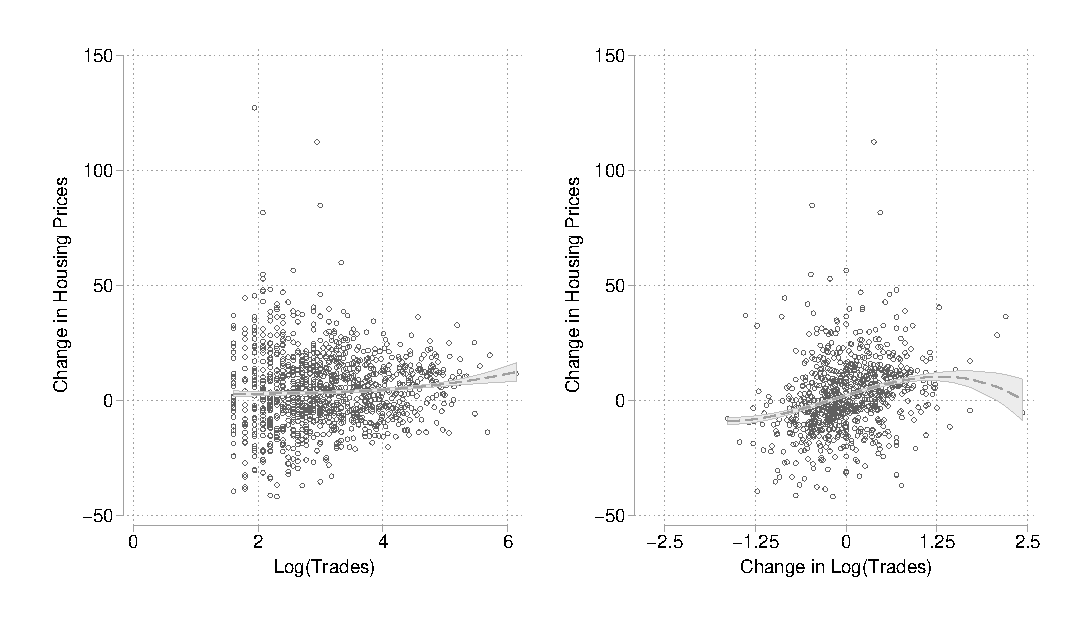
\includegraphics[width=1\textwidth]{../figures/corrmoderator.eps}
				\caption{How Closely Related is Number of Trades and Changes in Housing Prices? Dots are observations, line is fractional polynomial fit and area represents 95 pct. confidence interval of this fit. For number of trades the overall Pearson correlation with prices is $0.1$ ($n=4,199$), for the change variable it is $0.3$ ($n=3,100$). }
				\label{scatter}
			\end{figure}
			
			
			\begin{figure}
				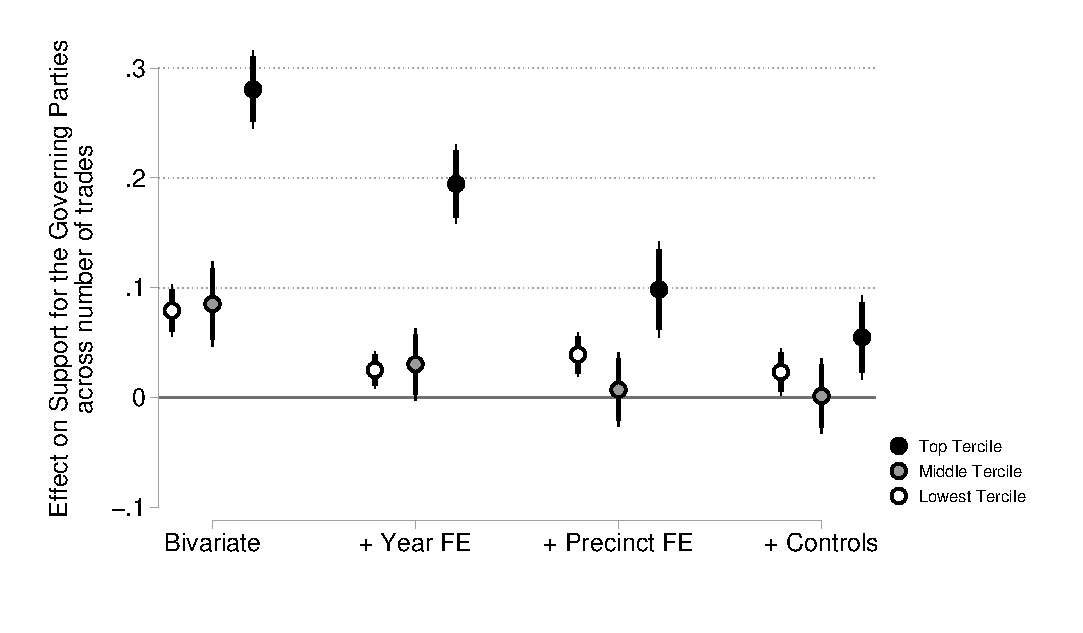
\includegraphics[width=0.7\textwidth]{../figures/localactivity_sup.eps}
				
				\caption{Interaction estimation using the binning estimator developed by Hainmueller, Mummolo and Xu (2016). The binning estimator is applied to all four specification presented in table \ref{predv}. }
				\label{terciles}
			\end{figure}
			
			\newpage
			
			\subsection{Some Additional Interactions in the Precinct-Level Data} \label{add_interaction}
				\setcounter{table}{0}
			\setcounter{figure}{0}
			
			In Model 1 of Figure \ref{addinter} we examine whether there is an interaction effect between the logged number of eligible voters and housing prices. We find no such interaction. Furthermore, even if we include this interaction the main results hold up in that the housing price by logged number of trades is statistically significant and of the same approximate size. This is reassuring, because it suggests that, as we hypothesized, it is local housing market activity rather than market size that moderates the impact of local housing prices.
			
			In model 2 of Figure \ref{addinter} we examine whether there is an interaction effect between local housing market activity and the effect of unemployment. We do identify such an interaction effect. The effect is positive, which implies that the negative effect of local unemployment on incumbent support decreases as local housing market activity increases. In particular, we find that moving from the 25th to the 75th percentile of log(trades) decreases the impact of the unemployment rate with 0.3 corresponding to a little less than 20 pct. of the average effect estimated in Table \ref{predv}.
			\begin{table}[htbp]\centering
\def\sym#1{\ifmmode^{#1}\else\(^{#1}\)\fi}
\caption{Some additional interactions} \footnotesize \label{addinter}
\begin{tabular}{l*{2}{c}}
\hline\hline
                    &\multicolumn{1}{c}{(1)}        &\multicolumn{1}{c}{(2)}        \\
\hline
$\Delta$ housing price&      -0.178\sym{*} &      -0.067\sym{*} \\
                    &     (0.071)        &     (0.030)        \\
[1em]
Log(trades)         &       1.943\sym{**}&      -0.446        \\
                    &     (0.447)        &     (1.121)        \\
[1em]
Log(Voters)         &       2.333        &                    \\
                    &     (1.688)        &                    \\
[1em]
$\Delta$ housing price $\times$ Log(trades)&       0.029\sym{**}&       0.028\sym{**}\\
                    &     (0.009)        &     (0.009)        \\
[1em]
$\Delta$ housing price $\times$ Log(Voters)&       0.014        &                    \\
                    &     (0.010)        &                    \\
[1em]
Log(Median income)  &      -0.850\sym{**}&      -0.834\sym{**}\\
                    &     (0.044)        &     (0.044)        \\
[1em]
Unemployment rate   &      -1.623\sym{**}&      -2.349\sym{**}\\
                    &     (0.190)        &     (0.351)        \\
[1em]
Unemployment rate $\times$ Log(trades)&                    &       0.205\sym{*} \\
                    &                    &     (0.086)        \\
[1em]
\hline Precinct FE  &$\checkmark$        &$\checkmark$        \\
[1em]
Year FE             &$\checkmark$        &$\checkmark$        \\
\hline
Observations        &        4179        &        4179        \\
RMSE                &       6.217        &       6.214        \\
\hline\hline
\multicolumn{3}{l}{\footnotesize Standard errors in parentheses}\\
\multicolumn{3}{l}{\footnotesize \sym{*} \(p<0.05\), \sym{**} \(p<0.01\)}\\
\end{tabular}
\end{table}

						
			\newpage
			
			\subsection{Precint-Level Results Without Estimated Precints} \label{calc}
				\setcounter{table}{0}
			\setcounter{figure}{0}
			
			As mentioned in the paper, 15 pct. of the electoral precincts merge or split up in different ways  across our period of study. For these precincts, we calculate vote returns using an interpolation method developed by Søren Risbjerg Thomsen, which is described at \texttt{\href{http://bit.ly/205OlPi}{bit.ly/205OlPi}}. To make sure that this procedure is not driving our results, Table \ref{calc} re-estimate our full model, including year and precinct fixed effects as well as economic controls, with and without the logged number og trades interaction, but without these estimated precincts. The results remain unchanged.  
			
			\begin{table}[htbp]\centering
\def\sym#1{\ifmmode^{#1}\else\(^{#1}\)\fi}
\caption{Main results excluding amalgamated precincts} \footnotesize \label{calculated}
\begin{tabular}{l*{2}{c}}
\hline\hline
                    &\multicolumn{1}{c}{(1)}        &\multicolumn{1}{c}{(2)}        \\
\hline
$\Delta$ housing price&       0.038\sym{**}&      -0.092\sym{**}\\
                    &     (0.010)        &     (0.035)        \\
[1em]
Median income (1000 DKK)&      -0.969\sym{**}&      -0.916\sym{**}\\
                    &     (0.052)        &     (0.052)        \\
[1em]
Unemployment rate   &      -2.117\sym{**}&      -1.723\sym{**}\\
                    &     (0.223)        &     (0.229)        \\
[1em]
Log(trades)         &                    &       2.299\sym{**}\\
                    &                    &     (0.518)        \\
[1em]
$\Delta$ housing price $\times$ Log(trades)&                    &       0.040\sym{**}\\
                    &                    &     (0.011)        \\
[1em]
\hline Precinct FE  &$\checkmark$        &$\checkmark$        \\
[1em]
Year FE             &$\checkmark$        &$\checkmark$        \\
\hline
Observations        &        3523        &        3523        \\
RMSE                &       6.559        &       6.500        \\
\hline\hline
\multicolumn{3}{l}{\footnotesize Standard errors in parentheses}\\
\multicolumn{3}{l}{\footnotesize \sym{*} \(p<0.05\), \sym{**} \(p<0.01\)}\\
\end{tabular}
\end{table}

			
			
		\end{document}


